%%%%%%%% ICML 2026 SUBMISSION (official icml2026 style kit) %%%%%%%%%%%%%%%%%
% Swap icml2026 -> icml2027 files when the ICML 2027 kit is released.

\documentclass{article}

% Recommended, but optional, packages for figures and better typesetting:
\usepackage{microtype}
\usepackage{graphicx}
\usepackage{subcaption}
\usepackage{booktabs} % for professional tables
\usepackage{placeins} % \FloatBarrier: keep body floats before the references
% looser float placement, so full-width floats can share a page top and leave no blank columns
\renewcommand{\topfraction}{0.9}\renewcommand{\dbltopfraction}{0.9}
\renewcommand{\bottomfraction}{0.8}\renewcommand{\textfraction}{0.07}
\renewcommand{\floatpagefraction}{0.7}\renewcommand{\dblfloatpagefraction}{0.7}
\setcounter{topnumber}{3}\setcounter{dbltopnumber}{3}\setcounter{totalnumber}{6}
\usepackage{bbold}
\usepackage{enumitem}

% hyperref makes hyperlinks in the resulting PDF.
% If your build breaks (sometimes temporarily if a hyperlink spans a page)
% please comment out the following usepackage line and replace
% \usepackage{icml2026} with \usepackage[nohyperref]{icml2026} above.
% \usepackage{hyperref}

% Attempt to make hyperref and algorithmic work together better:
\newcommand{\theHalgorithm}{\arabic{algorithm}}

% Use the following line for the initial blind version submitted for review:
\usepackage[nohyperref]{icml2026}

% For preprint, use
% \usepackage[preprint]{icml2026}

% If accepted, instead use the following line for the camera-ready submission:
% \usepackage[accepted]{icml2026}

\usepackage{amsmath}
\usepackage{amssymb}
\usepackage{mathtools}
\usepackage{amsthm}

% if you use cleveref..
\usepackage[capitalize,noabbrev]{cleveref}

%%%%%%%%%%%%%%%%%%%%%%%%%%%%%%%%
% THEOREMS
%%%%%%%%%%%%%%%%%%%%%%%%%%%%%%%%
\theoremstyle{plain}
\newtheorem{theorem}{Theorem}[section]
\newtheorem{proposition}[theorem]{Proposition}
\newtheorem{lemma}[theorem]{Lemma}
\newtheorem{corollary}[theorem]{Corollary}
\theoremstyle{definition}
\newtheorem{definition}[theorem]{Definition}
\newtheorem{assumption}[theorem]{Assumption}
\theoremstyle{remark}
\newtheorem{remark}[theorem]{Remark}

% Todonotes is useful during development; for the submission, comment out the
% second line and uncomment the first to hide all notes.
%\usepackage[disable,textsize=tiny]{todonotes}
\usepackage[textsize=tiny]{todonotes}

%%%%%%%%%%%%%%%%%%%%%%%%%%%%%%%%
% PROJECT MACROS
%%%%%%%%%%%%%%%%%%%%%%%%%%%%%%%%
\newcommand{\tvc}{TVC}
\newcommand{\vbar}{\bar v}
\newcommand{\sbar}{\bar s}
\newcommand{\Bbar}{\bar B}
\newcommand{\philo}{\varphi_{\mathrm{lo}}}
\DeclareMathOperator{\E}{\mathbb{E}}

% The \icmltitle you define below is probably too long as a header.
% Therefore, a short form for the running title is supplied here:
\icmltitlerunning{Truthful Verified Credit (TVC)}

\begin{document}

\twocolumn[
  \icmltitle{Truthful Verified Credit:\\
    Making Truth Dominant for Exploring Agents}

  % Author information is removed automatically in the blind version
  % (no [accepted] option). Fill in for the camera-ready version.
  \icmlsetsymbol{equal}{*}

  \begin{icmlauthorlist}
    \icmlauthor{Nhan Nguyen}{inst}
  \end{icmlauthorlist}

  \icmlaffiliation{inst}{Independent Researcher}

  \icmlcorrespondingauthor{Nhan Nguyen}{vinhnhan1999bc@gmail.com}

  % Keywords populate PDF metadata only (not shown in the document).
  \icmlkeywords{Multi-Agent Reinforcement Learning, Mechanism Design, Incentive Design, Truthful Communication, Multi-Agent Pathfinding}

  \vskip 0.3in
]

% Use ONE of the following lines. DO NOT remove the command.
\printAffiliationsAndNotice{}  % no special notice (required even if empty)
% \printAffiliationsAndNotice{\icmlEqualContribution}

\begin{abstract}
  % ICML: a single paragraph, ideally 4--6 sentences.
  Learning agents that share claims are increasingly rewarded for being relied on, but credit for attention rewards being followed, not being honest.
  We show that such credit breeds hype, and that under congestion hype is a social dilemma: it benefits each agent yet ruins the group.
  We propose truthful verified credit (\tvc{}), which rewards only verified value, adds a bonus for every checked claim, and fines audited false claims, and we derive the audit fine needed to outweigh the private outside gain of a lie.
  In a multi-agent bandit, \tvc{} cuts exaggeration from over 90\% of reports to below 1\% at welfare comparable to popularity credit.
  In multi-robot pathfinding on POGEMA, it cuts the hype rate of self-interested learners from 99\% to 0.2\% and triples lifelong throughput, and lying collapses within a factor of two of the predicted fine threshold.
  % Numbers: 10 seeds, 150 episodes (logs/fake_jams_lam.md, fake_jams_pogema.md, fake_jams_fine.md).
\end{abstract}

\section{Introduction}
\label{sec:intro}

In a review of FDA records for twelve antidepressants, 94\% of the trials in the
published literature were positive, against 51\% in the FDA's own analysis, and
the published effect sizes were 32\% larger overall \citep{turner2008selective}.
The pattern is not confined to medicine: in a set of peer-reviewed
social-science experiments, strong results were 60 percentage points more likely
to be written up than null results \citep{franco2014publication}. Selection also
acts inside a study. Comparing trial protocols with their publications, 40--62\%
of trials had at least one primary outcome changed, introduced or omitted, and
statistically significant outcomes were more likely to be fully reported
\citep{dwan2008systematic}. This is publication bias and reporting bias, the
file drawer problem of \citet{rosenthal1979file}, and it needs no fraud: small
studies, flexible analyses and competing interests already make many published
findings likely to be false \citep{ioannidis2005why}, and incentives that reward
publication can select for weak methods without anyone cheating deliberately
\citep{smaldino2016natural}. Authors respond to the credit they receive, and a
literature that credits positive, attention-getting results teaches them to
report only those.

Behind these figures lies a problem of rewarding exploration. Agents that search
on behalf of a group bear the cost of exploring, but what they find can save
everyone else the same work, so a group gains only when its members explore and
then report truthfully what they find. Models of the division of cognitive labor show that
the reward for discovery shapes which problems a community chooses to pursue
\citep{kitcher1990division, strevens2003priority}, and the same dependence
appears when a planner decides what to disclose to agents whose own experiments
create the information others rely on \citep{kremer2014wisdom}. How to reward
such exploration is a credit assignment problem, the problem of crediting each
agent for its own contribution to a shared return \citep{foerster2018coma}. A
growing family of methods now rewards agents directly for their effect on others:
social-influence rewards credit an agent for changing other agents' actions
\citep{jaques2019social}, and learned incentive functions let agents reward one
another to shape behavior \citep{yang2020lio}. Whenever credit flows to whoever
is relied on, it determines not only how much a group explores but whether its
members report what they find honestly.

Theory explains why such failures persist. Conflicts of interest limit how much
information survives strategic communication \citep{crawford1982strategic},
receivers who take messages at face value are deceived by inflated language
\citep{kartik2007credulity}, and a sender who controls what is revealed can
steer a rational receiver's choice \citep{kamenica2011bayesian}. Citation counts
can be inflated outright, as when editors pressure authors to cite their journal
\citep{wilhite2012coercive}, and reward-maximizing learning agents with no
built-in intent to deceive have been observed to distort their signals once
distortion is profitable \citep{alon2023disinformation}.

Intuitively, there are six common designs for the credit. However, each falls
short.

\paragraph{Credit from the shared return.}

Every agent receives the group's return, the default in cooperative multi-agent
learning, where a shared reward does not say which agent contributed to it
\citep{foerster2018coma}. An explorer bears the full cost of exploring, while its
own contribution to a return shared by many agents is hard to discern, so
exploring and reporting are under-supplied. It also cannot tell a true report
from an untruthful one, since both change the shared return only through what
others later do with them.

\paragraph{Credit for keeping exploring.}

Explorers are credited for each exploration, whatever it yields. This sustains exploration, but it is blind to what is reported: a true report, an exaggerated one and silence all earn the same, so honesty has no advantage, and credit is spent on explorations whose findings never reach the group. Untruthful reports then harm the group that relies on them: they inflate apparent effects, as in
the antidepressant trials above \citep {turner2008selective}, and they add to avoidable waste in research \citep{chalmers2009avoidable}.

\paragraph{Credit for only being followed (Popularity credit).}

Explorers are credited for attention, not accuracy. It encourages agents to explore
more as they get rewarded more. A inflated claim attracts followers as readily as a real one, so exaggeration is profitable and a learner finds it. This is the same situation that celebrities may promote low-quality products without careful consideration, prioritizing their own financial gain over the well-being of consumers or reporting bias aforementioned.

\paragraph{Credit for only being accurate.}

Explorers are credited only for the verified gain of those who rely on a claim. This
leaves a true report that nobody uses with nothing, which is the incentive
behind the file drawer, and a community can stall in a state where no one
reports because no one listens. Such credit also never checks an unused claim,
so truth, exaggeration and silence all earn the same. Accuracy-based remedies
from the literature do not close this gap: peer prediction makes honesty an
equilibrium rather than a dominant strategy \citep{miller2005peer}, and proper
scoring rules require the outcome to be observed \citep{gneiting2007strictly}.

\paragraph{A cost for lying alone.}

A fine charged when an audit finds a report false \citep{becker1968crime}. It
helps reduce lying rate of the agents. Nevertheless, it is not enough either: a
lie that is followed still collects the followers' credit, so the fine has to
outbid it, and a true report that nobody follows still earns nothing, so truth
is no better than silence. Moreover, a lie can be profitable outside the credit channel,
as when a hyped claim attracts followers whose attention benefits the claimant,
so the penalty must outweigh a temptation the designer does not control. With
smooth lying costs, \citep{kartik2009StrategicCommunicationLying} shows that
truthful reporting is never an equilibrium, and that inflation shrinks with cost
intensity but persists.

\paragraph{Reputation without credit.}

Receivers stop following senders who were wrong before, and give nothing. This
learns only from claims that were checked, and a claim that nobody follows is
never checked, so unused lies leave a sender's reputation untouched. It also
gives an honest explorer no reason to report: a new sender starts without trust
and may not be followed, so a true report can go unused and earn nothing.

These failures set our goal. We ask for a credit rule under which reporting the
truth is each agent's best action whatever the others do with the report,
including when a lie or a withheld result carries a private gain the designer
neither funds nor observes. Because receivers in learning systems, like
readers of a literature, keep changing how they respond, the guarantee cannot
rest on an equilibrium or on a model of receiver behavior; it must hold for
every receiver rule, so truth must beat the response most favorable to a lie.

Our key idea is to reward only verified value and to make every claim face a
check. We propose Truthful Verified Credit (\tvc{}), which wraps any host credit
scheme with three parts, each rewarding truth at least as much as a lie in every
case. Verified gain credit rewards the realized improvement of those who rely on a
report, capped, and only when the report passes verification. A checked score
bonus rewards every report that is checked, whether by a follower or by an
independent random audit, so a true report, including a negative one, earns
credit even when nobody acts on it. An audit fine is charged when an audit finds
a report false, and we derive the fine needed to outweigh a lie's outside gain.

We study \tvc{} in two settings. In a multi-agent bandit, where agents search
arms of unknown value on behalf of a group, popularity credit drives over
90\% of reports to be exaggerated, while \tvc{} brings it below one percent at
comparable welfare. In a congestion setting built on a multi-agent pathfinding (MAPF)
benchmark \citep{skrynnik2025pogema}, robots can post fake jams to clear their
own routes: self-interested learners lie at 91--99\% of opportunities without
credit, \tvc{} holds the rate near 0.2\%, and throughput rises about threefold.

% We summarize our contributions as follows.
% \begin{itemize}
%   \item We formalize collective exploration with reliance-based credit and show that rewarding attention breeds hype and silence; when information drives congestion, hype becomes a social dilemma in which every agent hyping lowers group output by 65\% (\cref{sec:problem,sec:experiments}).
%   \item We propose \tvc{}, show that truth earns more than any lie for every receiver rule, and show by ablation that each of its parts is needed (\cref{sec:why,sec:experiments}).
%   \item We derive the audit fine required when lies carry outside gains and confirm the predicted threshold empirically (\cref{eq:fine,sec:experiments}).
%   \item We evaluate \tvc{} in a multi-agent bandit and in multi-agent pathfinding, and report its limits: \tvc{} elicits truth rather than usefulness, so its unconditional bonus can encourage reports that carry no value, and it raises welfare only where honest information changes what others do (\cref{sec:experiments,sec:conclusion}).
% \end{itemize}

\section{Related Work}
\label{sec:related}

\paragraph{Credit among learning agents.}
Credit assignment in cooperative multi-agent reinforcement learning asks how to credit each agent for its share of a shared return. Payoff design gives each agent a payoff that serves the group objective \citep{wolpert2001optimal}, counterfactual baselines estimate an agent's marginal contribution \citep{foerster2018coma}, and value decomposition splits a team value into per-agent values \citep{sunehag2018value,rashid2018qmix}. These methods assume cooperative agents who report honestly. With mixed motives, as in sequential social dilemmas \citep{leibo2017multi}, shaping the reward changes behavior: inequity aversion promotes cooperation \citep{hughes2018inequity}, social-influence rewards credit an agent for changing others' actions \citep{jaques2019social}, and gifting or learned incentives let agents reward one another \citep{lupu2020gifting,yang2020lio}. These incentives reward being relied on, not being right, so an agent can raise its credit by exaggerating. This is an instance of reward hacking, where optimizing a proxy reward degrades the true objective \citep{amodei2016concrete,skalse2022defining}. \tvc{} is a rule for what to reward, and it can replace that credit.

\paragraph{Strategic communication.}
Conflicts of interest limit what cheap talk can convey \citep{crawford1982strategic}. Receivers who take messages at face value are deceived by inflated language \citep{kartik2007credulity}, a sender who controls what is revealed can steer a rational receiver \citep{kamenica2011bayesian}, and with a smooth cost of lying, inflation falls but persists \citep{kartik2009StrategicCommunicationLying}. Learning agents with no intent to deceive distort their signals once distortion is profitable \citep{alon2023disinformation}. These works analyze equilibria against a model of the receiver. We ask for dominance against every receiver rule.

\paragraph{Truthful elicitation and verification.}
Proper scoring rules need the outcome to be observed \citep{gneiting2007strictly}, and peer prediction \citep{miller2005peer,shnayder2016informed,feng2022peer,gao2019incentivizing} makes honesty an equilibrium and not a dominant strategy. With costly verification, the optimal mechanism checks only some reports, and a cost of lying lowers how often \citep{benporath2014OptimalAllocationCostly}, in line with deterrence by probabilistic enforcement \citep{becker1968crime}. \tvc{} audits a random sample, which makes truth dominant, and its follower gain is a VCG-style externality payment \citep{vickrey1961counterspeculation,clarke1971multipart,groves1973incentives} adapted to receivers who act by their own rule.



\section{Problem Setting}
\label{sec:problem}
We consider a multi-agent bandit game with private payoff. 
% We choose this game setting as it is the simple game where exploration is costly and private, a finding helps others, and receivers cannot check a claim before acting on it. It also has a ground truth the designer can audit, so lying, silence and reliance credit can all be measured and the payoffs stay simple enough to prove truth dominates.
There are $N$ agents and $K$ arms. Arm $k$ has a value $v_k>0$, drawn i.i.d.\ from a distribution $F$ with finite mean and fixed within an episode. The mean value is $\vbar=\frac1K\sum_k v_k$, and all credit amounts below are in units of $\vbar$. Play lasts $T$ rounds. Agent $i$ holds a set of known arms $\mathcal K_i^t\subseteq\{1,\dots,K\}$ with current best value $b_i^t=\max_{k\in\mathcal K_i^t}v_k$.

In each round, a free agent $i$ chooses through its policy $\pi_i$ to \emph{explore}, pulling an unknown arm and adding it to $\mathcal K_i$, or to \emph{exploit}, pulling its best known arm. Exploring costs $c\ge0$. Agent $i$ observes the payoff of its own pulls only, and its payoff $u_i^t$ is the value of the pulled arm, minus $c$ when exploring. On discovering arm $k$ in round $t$, agent $i$ observes $y_i^t=v_k e^{\epsilon_i^t}$ with $\epsilon_i^t\sim\mathcal N(0,\sigma^2)$, drawn i.i.d., is the observation noise: a random error that the explorer picks up when it discovers an arm. We write $\theta_i^t=v_k$ for the true value behind this observation. Pulling an arm yields its true value; only the discovery observation is noisy.

After discovering an arm, agent $i$ may post a public claim $m_i^t\in\{\varnothing\}\cup\mathbb R_{>0}$, where $\varnothing$ is silence. Posting a claim cost $\xi\ge0$. The claim is \emph{truthful} if $m_i^t=y_i^t$. We denote $\kappa_i^t=m_i^t/y_i^t$ is inflation rate. Each free agent $j$ that did not explore then chooses whom to follow, $d_j^t=\rho_j(h_j^t,m^t)\in\{0\}\cup\{1,\dots,N\}\setminus\{j\}$, where $0$ means nobody, $h_j^t$ is $j$'s private history and $m^t=(m_1^t,\dots,m_N^t)$. Following $i$ commits $j$ to $i$'s arm for $L$ rounds. The \emph{receiver rule} $\rho_j$ is an arbitrary function: it may be a fixed heuristic, a Bayesian update, a learning policy or an adversary. We assume no rationality and no equilibrium among receivers. The follower's gain over its own best is
\begin{equation}
  g_{ji}^t=L\,\big(\theta_i^t-b_j^t\big)^{+}.
  \label{eq:gain}
\end{equation}

A receiver cannot check a claim before it acts on it; it learns $\theta_i^t$ exactly only by following. 

\paragraph{Reward.}
A sender maximises a mixed-motive reward in which it weighs the others' mean payoff $\bar u_{-i}^t$ by the \emph{prosocial weight} $\lambda\in[0,1]$, where $\lambda=0$ is a selfish sender and $\lambda=1$ a fully cooperative one,
\begin{equation}
  r_i^t=(1-\lambda)\,u_i^t+\lambda\,\bar u_{-i}^t-\xi\,\mathbb 1[m_i^t\neq\varnothing]+C_i^t,
  \label{eq:reward}
\end{equation}
where $\bar u_{-i}^t=\frac1{N-1}\sum_{j\neq i}u_j^t$ is the mean payoff of the other agents.

\paragraph{Outside gain.}
A claim can also change the sender's reward outside the credit, because believers act on it. Relative to a truthful claim, a lie raises the liar's own payoff $u_i^t$ by $G_1\ge0$, for example the citations a researcher gains, and lowers the others' mean payoff $\bar u_{-i}^t$ by $D_1\ge0$, for example the time they waste on a misleading approach, both per lie and in units of $\vbar$. Formally, $G_1=\mathbb E[u_i^t\mid\text{lie}]-\mathbb E[u_i^t\mid\text{truthful claim}]$ and $D_1=\mathbb E[\bar u_{-i}^t\mid\text{truthful claim}]-\mathbb E[\bar u_{-i}^t\mid\text{lie}]$, where the expectation is over how the receivers respond. A sender's payoff changes with a claim only through what others do, so $G_1>0$ needs a setting in which others' actions affect it. We take the largest values over receiver rules. The sender feels a share $1-\lambda$ of its gain and a share $\lambda$ of the damage, so a lie changes the part of its reward that does not come from the credit by the \emph{outside gain}
\begin{equation}
  \Gamma=(1-\lambda)G_1-\lambda D_1 .
  \label{eq:gamma}
\end{equation}
The designer neither observes nor provides $\Gamma$, and we assume $\Gamma\ge0$. The posting cost $\xi$ is borne by truth and lie alike, so it does not enter $\Gamma$; it matters only when a claim is compared with silence.

% ---------------------------------------------------------------------------------------------------
% \subsection{Credit for being relied on}
% \label{sec:credit}

% A \emph{host} credit scheme gives sender $i$ an amount $H_i^t$ that grows with reliance on $i$, and an agent maximizes its return under $r_i^t$ in \cref{eq:reward}. Two basic schemes are
% \begin{align}
%   H_i^t&=\beta\,\big|\{j:d_j^t=i\}\big| &&\text{(popularity)},\\
%   H_i^t&=\gamma\textstyle\sum_{j:\,d_j^t=i}L\,(\theta_i^t-b_j^t) &&\text{(accuracy)},
% \end{align}
% and social-influence rewards \citep{jaques2019social} and learned incentives \citep{yang2020lio} act like the first. All of them give credit only through reliance: $H_i^t=0$ whenever no one follows $i$.

% % ---------------------------------------------------------------------------------------------------
% \subsection{Why reliance credit fails}
% \label{sec:failure}

% Call a receiver profile \emph{monotone} if raising $m_i^t$ never makes a receiver stop following $i$, which holds for naive, calibrated and most learned rules.

% \paragraph{Hype.}
% Under popularity credit and a monotone profile, any inflation $m'>y_i^t$ weakly raises $H_i^t$, and strictly so whenever some receiver's threshold lies in $(y_i^t,m']$. Truth is then not a best response as soon as the added followers are worth more than the cost of the claim. Popularity rewards a fake claim and a real one alike, because both attract followers, so a learner finds inflation.

% \paragraph{Silence.}
% Because $H_i^t=0$ for an unfollowed claim, a true claim that nobody follows (for example $\theta_i^t\le b_j^t$ for all $j$, so there is nothing to gain) earns $0-c$, while silence earns $0$. Silence is strictly better whenever $c>0$, and equal otherwise, so a community can stall where no one reports because no one listens. Accuracy credit has this flaw as well, and a second one: an unfollowed claim is never checked, so truth, any lie and silence all earn the same. It is truthful only weakly.

% \paragraph{Outside gain.}
% If $\Gamma>0$, a lie is profitable with no credit at all. Any credit rule that rewards only verified value must also overcome $\Gamma$, and the amount it needs depends on a quantity the designer does not control.

% \paragraph{Social dilemma.}
% When information drives congestion, $\Gamma>0$ makes lying individually dominant, yet the harm $D_1$ it causes lowers the group's welfare $W=\frac1{\vbar}\sum_{i,t}u_i^t$. Lying then fits a social dilemma: every agent gains by it, but all lying leaves the group worse off than all honest.

% % ---------------------------------------------------------------------------------------------------
% \subsection{Design goal}
% \label{sec:goal}

% We want a credit $C_i^t$ that replaces $H_i^t$ in \cref{eq:reward}. Let $R_i(m)$ be sender $i$'s expected reward for claim $m$, given its observation $y_i^t$, taken over the audit draws only.

% \begin{definition}[Receiver-robust truthfulness]
%   \label{def:rrt}
%   Truthful reporting is \emph{receiver-robustly dominant} if there is a margin $\Delta>0$ such that, for every receiver profile $(\rho_j)_j$, every history and every claim $m\ne y_i^t$ (silence included), $R_i(y_i^t)-R_i(m)\ge\Delta\vbar$.
% \end{definition}

% The definition has three consequences. First, it is a dominance property: it holds against every receiver rule, so it needs no model of how receivers respond and survives their learning. Second, $R_i$ includes the outside gain $\Gamma$, so the margin holds against a lie that gains outside the credit channel. Third, the margin $\Delta$ is explicit, so it can be used to size the audit fine.

% We pursue this goal under four assumptions on the channel.
% \begin{enumerate}
%   \item \emph{Separability.} Given the receivers' actions, $u_i^t$ does not depend on $m_i^t$. Claims affect $i$ only through $C_i^t$ and through the receivers' behaviour.
%   \item \emph{Unforgeable verification.} A checked claim reveals $\theta_i^t$ exactly, and followers cannot misreport it.
%   \item \emph{Independent audits.} $a_i^t$ is independent of the claims, the receivers' choices and the history.
%   \item \emph{Lie separation.} A truthful claim is verified, and every other claim fails the tolerance $\tau$.
% \end{enumerate}
% We do not assume limited liability: the credit may be negative. We also ask for a bounded cost, $\E\big[\sum_{i,t}(C_i^t)^{+}\big]\le\mathcal B$ for a budget $\mathcal B$, and no loss of welfare $W$ when all agents report truthfully. The next section gives a credit that meets \cref{def:rrt} under these assumptions.

\section{Truthful Verified Credit}
\label{sec:method}
% With the problem defined in \cref{sec:problem}, we introduce the mechanism of \tvc{}. It has three parts, and each answers one failure of reliance credit mentioned. We first introduce the three components of the proposed mechanism. We then explain how the mechanism addresses the credit assignment problem and why each component is essential. Finally, we illustrate its operation through a simple example.

\subsection{Verified externality credit}
\label{sec:ext}

Popularity credit rewards a fake claim and a real one alike, because both attract followers. Let $\mathcal F_i^t=\{j:\,d_j^t=i\}$ be the \emph{follow set} of sender $i$: the receivers $j$ that follow $i$'s claim in round $t$ and so observe $\theta_i^t$ exactly. \tvc{} instead credits the followers' realized gain \cref{eq:gain}, and only for a claim that is verified:
\begin{equation}
  \sum_{j\in\mathcal F_i^t} V_i^t\,\min\!\big(g_{ji}^t,\,\Bbar\vbar\big).
  \label{eq:ext}
\end{equation}
Here $V_i^t=\mathbb{1}\big[\,|m_i^t/\theta_i^t-1|\le\tau\,\big]$ is the verification gate: it equals $1$ when the claim lies within a tolerance $\tau\ge0$ of the true value $\theta_i^t$, and $0$ otherwise. The tolerance $\tau$ is set above the honest noise level $\epsilon$, so a truthful claim passes the gate and any claim outside the tolerance is blocked. Every $j\in\mathcal F_i^t$ learns $\theta_i^t$ exactly on committing, so a followed claim ($\mathcal F_i^t\neq\emptyset$) is checked at no cost to the designer. 

The gain $g_{ji}^t$ is the externality of $i$'s report on $j$ relative to $j$ staying put, as in a VCG mechanism \citep{vickrey1961counterspeculation,clarke1971multipart,groves1973incentives}. A lie that is followed fails the gate $V_i^t$ and earns no gain credit, so attracting followers with an inflated claim no longer brings a gain. The cap $\Bbar\vbar$, with $\Bbar>0$ a design parameter in units of the mean value $\vbar$, limits what one follower can add, so a single lucky find cannot dominate the sender's return. Each receiver follows at most one claim, so the cap also bounds the cost: the gain term adds at most $N\Bbar\vbar$ per round.

\subsection{Checked score bonus}
\label{sec:bonus}

Gain credit alone leaves silence as a best response: a true claim that nobody follows earns nothing, exactly like staying silent. \tvc{} therefore gives every checked claim a bonus that peaks at the truth,
\begin{equation}
  \chi_i^t\,\eta\,\vbar\,S\big(m_i^t,\theta_i^t\big),
  \label{eq:bonus}
\end{equation}
where $\eta>0$ is the bonus weight and the score is a Gaussian in the log error with width $w>0$,
\begin{equation}
  S(m,\theta)=\exp\!\Big(-\frac{(\ln m-\ln\theta)^2}{2w^2}\Big).
  \label{eq:score}
\end{equation}
A claim is \emph{checked} when it is audited or followed,
\begin{equation}
  \chi_i^t=\mathbb 1[m_i^t\neq\varnothing]\,\max\big(a_i^t,f_i^t\big),
  \qquad
  f_i^t=\mathbb 1\big[\mathcal F_i^t\neq\emptyset\big],
  \label{eq:checked}
\end{equation}
where $f_i^t$ indicates that someone followed $i$, and $a_i^t$ indicates a random audit of the claim, drawn independently of the claim and of the receivers,
\begin{equation}
  a_i^t\sim\mathrm{Bernoulli}(p),\qquad p\in(0,1].
  \label{eq:audit}
\end{equation}
A claim is thus checked either by a follower or by a random audit, and the audit is what reaches claims nobody follows. Because the audit is independent of the claim and of the receivers, a true claim earns at least $p\,\eta\vbar$ in expectation however receivers behave, and this is strictly more than silence, which earns $0$. This holds for a bad find as well, so reporting a low-value find is no longer a loss. The score is $1$ at the truth and below $\sbar=\sup_{|m/\theta-1|>\tau}S(m,\theta)<1$ for every claim that fails the tolerance, so inflation cannot raise the bonus.

\subsection{Audited lying cost}
\label{sec:cost}

The first two parts leave a lie with a small payoff, the bonus up to $\eta\sbar\vbar$, and say nothing about an outside gain $\Gamma$, the net private benefit a lie brings its sender outside the credit channel, for example a false report that steers others away from something the sender wants for itself. \tvc{} therefore fines every audited claim that fails verification, with a fine $\varphi\ge0$ in units of $\vbar$:
\begin{equation}
  a_i^t\,(1-V_i^t)\,\mathbb 1[m_i^t\neq\varnothing]\,\varphi\,\vbar.
  \label{eq:cost}
\end{equation}
The fine is charged only on audits. An audit has probability $p$, independent of the claim and the receivers, so a lie costs $p\varphi\vbar$ in expectation whatever the receivers do, and the fine can be sized against $\Gamma$ without a model of the receivers (\cref{eq:fine}). Raising $\varphi$ lets the designer lower the audit rate $p$, which is the price of verification. We do not assume limited liability, so the net credit may be negative.

% We do not need to audit every claim. In an allocation problem with costly verification, \citet{benporath2014OptimalAllocationCostly} show that when lying carries a cost $\varphi$, the optimal mechanism is still a favored-agent mechanism, but its checking probability falls from $1$ to $1/(1+\varphi)$.


Together, the credit to sender $i$ in round $t$ is
\begin{equation}
  \begin{aligned}
    C_i^t ={}& \textstyle\sum_{j\in\mathcal F_i^t} V_i^t \min\!\big(g_{ji}^t,\Bbar\vbar\big) \\
    &+ \chi_i^t\,\eta\,\vbar\, S\big(m_i^t,\theta_i^t\big) \\
    &- a_i^t\big(1-V_i^t\big)\mathbb{1}\big[m_i^t\neq\varnothing\big]\,\varphi\,\vbar .
  \end{aligned}
  \label{eq:tvc}
\end{equation}
% \tvc{} wraps any existing credit scheme: the host's credit for a claim is replaced by \cref{eq:tvc}.

The algorithm for learning with \tvc{} per episode is shown in \cref{alg:tvc}, and the credit of one claim in \cref{alg:credit}.




% \begin{figure*}[t]
%   \centering
%   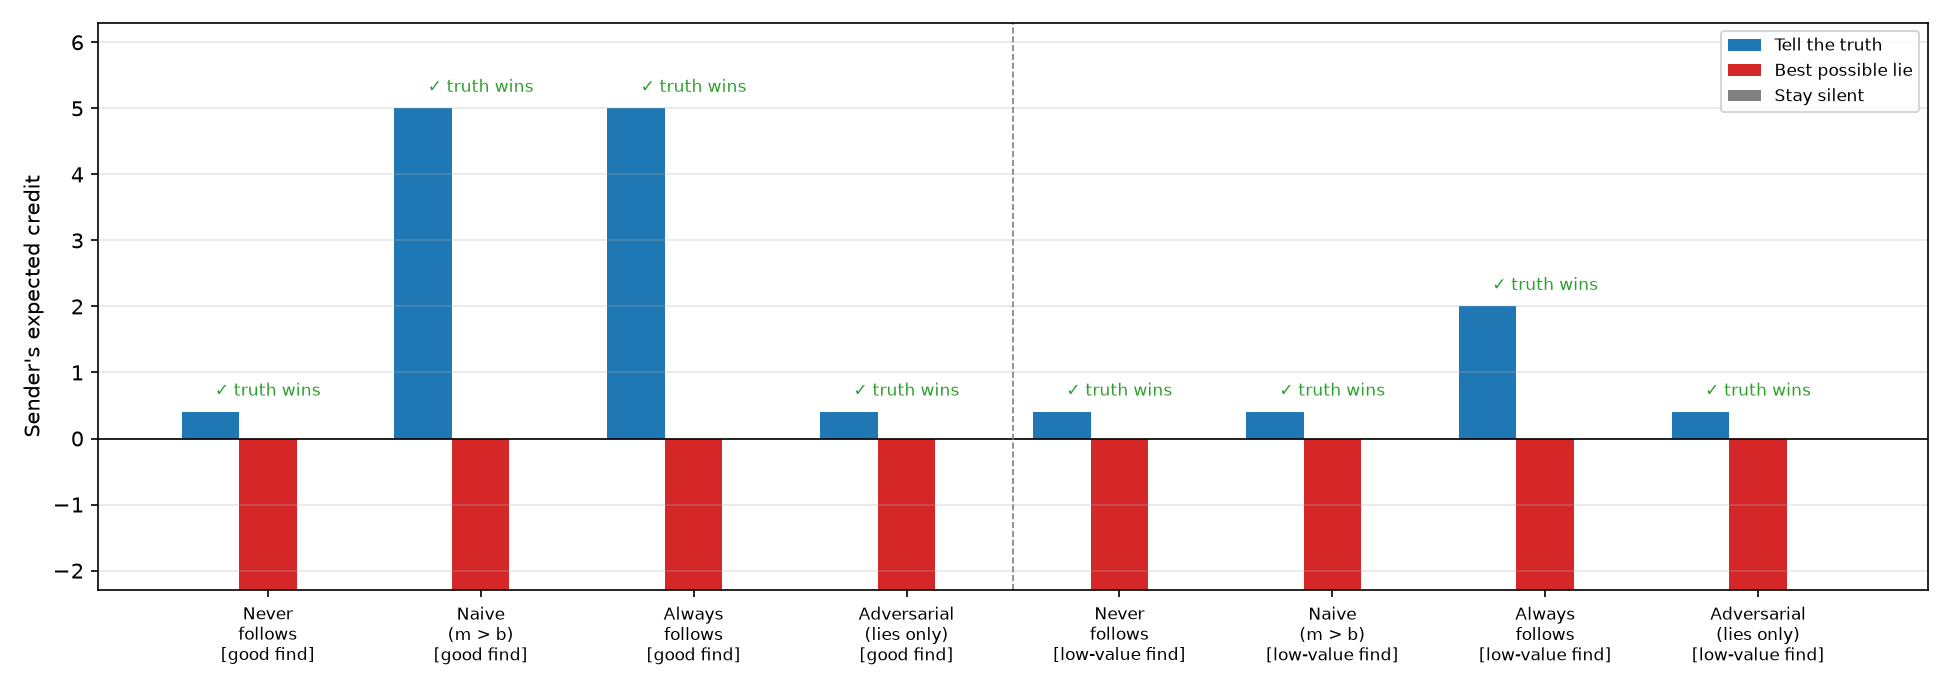
\includegraphics[width=\textwidth]{figures/honesty_every_case.png}
%   \caption{Truth against the best lie and silence under \tvc{}, for one sender, one receiver and one round. Each pair of groups of bars is a receiver rule (never follows, follows if the claim beats its best, always follows, or follows only lies) for a good find ($\theta=2$) and for a low-value find ($\theta=0.8$), with the follower's best value at $1$. Blue is the expected credit of the truthful claim, red is the best of the lies $\times0.9$, $\times1.1$, $\times1.5$ and $\times2$, and grey is silence, which earns $0$. Credit is in units of $\vbar$ and expected over the audit ($p=0.2$). Truth earns more than every lie and than silence in all eight cases.}
%   \label{fig:every_case}
% \end{figure*}

% \paragraph{Outside gain.}
% A lie can also be profitable for reasons outside the credit, a private gain $\Gamma$ that the designer neither observes nor rewards (defined in \cref{app:fine}). Truth then stays strictly dominant only if the fine exceeds $\philo=(\eta\sbar+\Gamma)/p-\eta$ (\cref{eq:fine}). A larger outside gain needs a larger fine, and so do fewer audits, in proportion to $1/p$.

% ---------------------------------------------------------------------------------------------------
\subsection{When \tvc{} is useful}
\label{sec:when}

\tvc{} is aimed at settings where four conditions hold together.
\begin{enumerate}
  \item \emph{Credit follows reliance.} Agents are credited for being followed or used, which rewards exaggeration and leaves a true report that nobody uses uncredited.
  \item \emph{Lying is profitable outside the credit.} Agents are not fully prosocial ($\lambda<1$), so a lie can bring a private gain that no reliance credit removes by itself.
  \item \emph{Lying harms others.} A false report misleads those who act on it and wastes their effort, and the group loses once several agents lie. Where receivers can decode exaggeration at little cost, hype costs little, and \tvc{} buys honest reports but not extra welfare.
  \item \emph{Claims can be audited at a cost.} Receivers cannot verify a claim before acting, but the designer can check a random sample at rate $p$.
\end{enumerate}
One of our testbeds meets all four (\cref{sec:experiments}). Other candidates, which we do not evaluate, are crowd-sourced traffic or robot-fleet reports, teams of language-model agents that build on one another's findings, and scientific credit through citations with sampled replication as the audit. When a condition fails, simpler designs may suffice: a shared return can work for nearly altruistic agents, and without any audit, peer prediction is the relevant regime.

% ---------------------------------------------------------------------------------------------------
% Job: make it implementable in a few lines. The credit of each claim is added to the return of the decision that
% produced it; everything else in the learner is unchanged.

\begin{algorithm}[t]
  \caption{Learning with \tvc{} (per episode)}
  \label{alg:tvc}
  \begin{algorithmic}
    \STATE Each sender decides to post a claim $m_i^t$ or stay silent; draw an audit $a_i^t\sim\mathrm{Bernoulli}(p)$ per claim
    \STATE Receivers act on the claims by their own rule; record who relied on which claim
    \STATE Mark a claim checked if it was audited or its outcome was observed by someone who relied on it
    \FOR{each claim}
      \STATE Compute $C_i^t$ by \cref{alg:credit}
      \STATE Add $C_i^t$ to the return of the decision that posted the claim
    \ENDFOR
    \STATE Update each sender's policy with its usual learning rule
  \end{algorithmic}
\end{algorithm}

\begin{algorithm}[t]
  \caption{\tvc{} credit of one sender in one round (the credit step of \cref{alg:tvc})}
  \label{alg:credit}
  \begin{algorithmic}
    \REQUIRE claim $m_i^t$ or silence $\varnothing$; follow set $\mathcal F_i^t$ and gains $g_{ji}^t$; audit draw $a_i^t$; true value $\theta_i^t$, revealed by a check; parameters $\tau,\Bbar,\eta,w,\varphi$
    \ENSURE credit $C_i^t$
    \IF{$m_i^t=\varnothing$}
      \STATE \textbf{return} $0$
    \ENDIF
    \STATE $\chi_i^t\leftarrow\max\big(a_i^t,\ \mathbb 1[\mathcal F_i^t\neq\emptyset]\big)$ \COMMENT{checked by an audit or a follower}
    \IF{$\chi_i^t=0$}
      \STATE \textbf{return} $0$ \COMMENT{an unchecked claim earns nothing}
    \ENDIF
    \STATE $V_i^t\leftarrow\mathbb 1\big[\,|m_i^t/\theta_i^t-1|\le\tau\,\big]$ \COMMENT{verification gate}
    \STATE $C_i^t\leftarrow\eta\,\vbar\,S\big(m_i^t,\theta_i^t\big)$ \COMMENT{score bonus}
    \IF{$V_i^t=1$}
      \STATE $C_i^t\leftarrow C_i^t+\sum_{j\in\mathcal F_i^t}\min\big(g_{ji}^t,\Bbar\vbar\big)$ \COMMENT{verified gain credit}
    \ELSIF{$a_i^t=1$}
      \STATE $C_i^t\leftarrow C_i^t-\varphi\,\vbar$ \COMMENT{fine for an audited false claim}
    \ENDIF
    \STATE \textbf{return} $C_i^t$
  \end{algorithmic}
\end{algorithm}

\todo{Parameter recipe: $\eta$ and $\Bbar$ in units of the mean value $\vbar$; $p$ from the audit budget; $\varphi = 2\philo$ from \cref{eq:fine}. Cost: one audit per $1/p$ claims.}

\section{Experiments}
\label{sec:experiments}

We study \tvc{} in two settings. In a multi-agent bandit, where agents search arms of unknown value on behalf of a group. In a congestion setting built on a multi-agent pathfinding (MAPF) benchmark \citep{skrynnik2025pogema}, robots can post fake jams to clear their own routes. 

\subsection{Experiment 1: Multi-agent Bandit} \label{subsec:experiment1}

\paragraph{Setup.}
$N=10$ agents search $K=50$ arms whose values are drawn i.i.d.\ from a lognormal distribution, in episodes of $T=100$ rounds, and each agent starts knowing one random arm. In each round a free agent either explores a random arm, at a cost of $0.5\vbar$, or exploits its best known arm. An explorer may post a claim about its find: silence, or the true value scaled by $\times1$ (truthful), $\times1.1$, $\times1.5$ or $\times2$. Free agents that did not explore follow the claim that beats their own best and stay committed for $L=3$ rounds. We use two kinds of receiver: naive receivers take a claim at face value, and calibrated receivers learn, for each sender, how far its claims exceed the truth, from the claims they have followed, with learning rate $0.3$. Explore and report decisions are learned by tabular REINFORCE (learning rate $0.1$, discount $0.9$, a running baseline per state), with the agent's own best and the value of its find as states.

\paragraph{Credit designs.}
We compare no credit, popularity credit ($2\vbar$ per follower), accuracy credit (the follower's signed gain), \tvc{} ($\tau=0.05$, $\Bbar=8$, $\eta=2$, $p=0.2$, $\varphi=8$, $w=0.05$), a shared return (every agent receives the group's mean payoff), credit for keeping exploring (a flat $3\vbar$ per exploration, matched to \tvc{}'s spend), a lying cost alone (audited false claims fined $\varphi$, nothing else given) and popularity credit with that fine. Reputation alone is no credit with calibrated receivers.

\paragraph{Metrics.}
Inflation (share of reports that are exaggerated), report rate (reports per exploration), misled follows (follows that lead to a worse arm), welfare (own payoff per round, in units of $\vbar$) and exploration rate. We report the mean over the last 100 of 1000 episodes with 95\% confidence intervals over 32 independent runs.

\paragraph{Results.}
\Cref{tab:bandit} compares the credit designs. Credit for being relied on breeds hype. With naive receivers, popularity credit raises inflation from 75.1\% (no credit) to 94.0\% and the share of misled follows from 25.5\% to 43.5\%. Accuracy credit does not remove it (68.9\% with naive and 85.1\% with calibrated receivers). \tvc{} brings inflation down to 0.3\% with naive and 0.4\% with calibrated receivers, raises the report rate to 99.6\%, and cuts misled follows to 0.2\%. A lying cost alone also removes most inflation (3.4\%), but half of the explorers choose to silent (report rate 50.0\%), and it has the lowest welfare (3.18 against 3.49 with no credit). Popularity credit with the same fine still has 38.4\% inflation. In welfare, \tvc{} (4.03) matches popularity credit (4.04) and exceeds no credit (3.49). The highest welfare comes from keeping exploring (4.28), which raises the exploration rate to 15.0\% against 3.0\% for \tvc{} but leaves inflation at 74.7\%. The shared return also raises exploration (23.3\%) but reaches the same welfare as \tvc{} (4.06) with 71.9\% inflation. \tvc{} therefore makes reports honest at no cost in welfare, but it does not by itself increase exploration. Calibrated receivers lower the cost of hype, as the conditions in \cref{sec:when} predict. With no credit they cut misled follows from 25.5\% to 7.6\%, and under popularity credit to 0.9\%, so popularity credit reaches the welfare of \tvc{} (4.02 against 3.96, within the intervals) at 92.2\% inflation.

% Multi-agent bandit, 1000 episodes, 32 runs, last 100 episodes (source: logs/bandit_run3.log, python -m tvc.bandit 1000).
% ICML: table captions go ABOVE the table.
\begin{table*}[t]
  \caption{Multi-agent bandit: credit designs compared (mean $\pm$ 95\% CI over 32 runs, last 100 of 1000 episodes). Inflation is the percentage of reports that are exaggerated, report is the percentage of explorations that are reported, misled is the percentage of follows that lead to a worse arm, and explore is the percentage of agent-rounds spent exploring. Welfare is the mean own payoff per agent per round, in units of the mean arm value. With calibrated receivers, \emph{None} is reputation only. \emph{Keeping exploring} gives a flat $3\vbar$ per exploration, \emph{Lying cost alone} fines audited false claims and gives nothing else, and \emph{Shared return} gives every agent the group mean payoff.}
  \label{tab:bandit}
  \centering
  \small
  \setlength{\tabcolsep}{4pt}
  \begin{tabular}{lccccc}
    \toprule
    Credit design & Inflation (\%)  & Report (\%)  & Misled (\%)  & Welfare ($\vbar$)  & Explore (\%) \\
    \midrule
    \multicolumn{6}{l}{\emph{Naive receivers}} \\
    None & $75.1 \pm 0.4$ & $80.2 \pm 0.3$ & $25.5 \pm 1.0$ & $3.486 \pm 0.104$ & $2.7 \pm 0.2$ \\
    Popularity & $94.0 \pm 0.5$ & $94.8 \pm 0.4$ & $43.5 \pm 1.1$ & $4.036 \pm 0.054$ & $4.5 \pm 0.2$ \\
    Accuracy & $68.9 \pm 2.4$ & $89.8 \pm 0.4$ & $13.7 \pm 1.2$ & $3.867 \pm 0.095$ & $2.9 \pm 0.2$ \\
    Shared return & $71.9 \pm 5.4$ & $80.1 \pm 4.7$ & $32.7 \pm 4.8$ & $4.055 \pm 0.145$ & $\mathbf{23.3 \pm 3.0}$ \\
    Keeping exploring & $74.7 \pm 1.1$ & $79.1 \pm 1.2$ & $41.3 \pm 1.8$ & $\mathbf{4.280 \pm 0.083}$ & $15.0 \pm 2.5$ \\
    Lying cost alone & $3.4 \pm 0.7$ & $50.0 \pm 2.9$ & $1.4 \pm 0.3$ & $3.177 \pm 0.114$ & $2.4 \pm 0.2$ \\
    Popularity + fine & $38.4 \pm 1.6$ & $85.0 \pm 2.4$ & $34.4 \pm 1.6$ & $3.859 \pm 0.070$ & $3.4 \pm 0.2$ \\
    \textbf{TVC} & $\mathbf{0.3 \pm 0.1}$ & $\mathbf{99.6 \pm 0.1}$ & $\mathbf{0.2 \pm 0.1}$ & $4.028 \pm 0.079$ & $3.0 \pm 0.2$ \\
    \midrule
    \multicolumn{6}{l}{\emph{Calibrated receivers (per-sender decoding)}} \\
    None & $75.1 \pm 0.5$ & $80.1 \pm 0.4$ & $7.6 \pm 0.5$ & $3.528 \pm 0.126$ & $2.5 \pm 0.3$ \\
    Popularity & $92.2 \pm 0.5$ & $93.4 \pm 0.5$ & $0.9 \pm 0.4$ & $4.023 \pm 0.078$ & $3.2 \pm 0.2$ \\
    Accuracy & $85.1 \pm 1.3$ & $90.6 \pm 0.4$ & $3.3 \pm 0.5$ & $3.993 \pm 0.097$ & $3.1 \pm 0.3$ \\
    Shared return & $68.0 \pm 6.8$ & $83.6 \pm 3.4$ & $3.3 \pm 0.7$ & $4.118 \pm 0.159$ & $\mathbf{23.7 \pm 3.6}$ \\
    Keeping exploring & $74.8 \pm 1.2$ & $79.2 \pm 1.1$ & $9.1 \pm 0.6$ & $\mathbf{4.358 \pm 0.079}$ & $15.1 \pm 2.6$ \\
    Lying cost alone & $3.5 \pm 0.7$ & $50.4 \pm 3.6$ & $1.3 \pm 0.2$ & $3.045 \pm 0.128$ & $2.2 \pm 0.3$ \\
    Popularity + fine & $33.4 \pm 2.3$ & $85.4 \pm 2.5$ & $2.5 \pm 0.4$ & $3.877 \pm 0.094$ & $2.5 \pm 0.2$ \\
    \textbf{TVC} & $\mathbf{0.4 \pm 0.1}$ & $\mathbf{99.6 \pm 0.2}$ & $\mathbf{0.2 \pm 0.1}$ & $3.963 \pm 0.081$ & $2.9 \pm 0.2$ \\
    \bottomrule
  \end{tabular}
\end{table*}


\subsection{Experiment 2: MAPF with fake jams} \label{subsec:experiment2}

\paragraph{Setup.}
We use POGEMA's lifelong pathfinding task \citep{skrynnik2025pogema} with soft collisions on a $3\times3$ layout of $5\times5$ rooms joined by 1-cell doorways, with 12 robots, observation radius $3$ and $256$ steps. Robots move by greedy descent on a distance map, so the only learned decision is whether to post a claim that a doorway they can see is jammed. We define the ground truth that a doorway is jammed when at least $3$ robots are within $2$ walking steps of it. Receivers that believe a claim avoid that doorway for $20$ steps, and a claim expires after $20$ steps. A claim is checked by a robot that passes the doorway, or by an audit. Naive receivers take claims at face value, and sceptical receivers learn per-sender trust from the checks they see (learning rate $0.3$).

\paragraph{Mixed motive.}
A robot's reward is $(1-\lambda)$ times its own deliveries plus $\lambda$ times the others' mean deliveries, minus a cost per claim posted, plus credit. A lie, a fake jam on its own route, gains the liar when believers leave that route and costs the others their detours. The per-believer gain, harm and benefit that enter the learning signal are calibrated from short runs with hand-set policies, and the temptation is therefore a modelling choice, not an emergent property. Claim policies are learned by tabular REINFORCE.

\paragraph{Credit designs.}
No credit, popularity credit ($1$ per believer), accuracy credit (the steps a believer saves, negative for a fake jam), \tvc{} ($\tau=0.05$, $\Bbar=8$, $\eta=2$, $p=0.2$, $\varphi=15$), reputation (no credit, sceptical receivers) and a shared return ($\lambda=(N-1)/N$).

\paragraph{Metrics.}
We report the lie rate (the share of opportunities on which a robot posts a fake jam on its own route), the useful-report rate (the share of real jams elsewhere that it reports), POGEMA's throughput (deliveries per step, summed over the 12 robots) and the credit given, as the mean over the last 50 of 150 episodes, with 95\% confidence intervals over 10 seeds.

\paragraph{Questions.}
We ask  questions. Does lying harm the group, so that honest reports are worth rewarding? Does \tvc{} remove lying and raise throughput compared with the other credit designs? Does it do so at every prosocial weight?.

\paragraph{Lying harms the group.}
We first check that lying is costly for the group, because only then is it worth rewarding honest reports. We fix the claim policies instead of learning them. The first $k$ of the 12 robots post a fake jam whenever a doorway on their own route is free, the others report real jams, and no credit is given. We run 10 batches of 20 episodes for each $k$, with 95\% confidence intervals over batches. With naive receivers, group deliveries per robot per episode fall from 5.8 with no liars to 1.9 with 12 (\cref{fig:hype}), and the share of detours that were for fake jams rises from 0.31 at $k=1$ to 0.95 at $k=12$. One liar gains 3.5 deliveries over its honest peers while the others lose 0.5, so a single lie mostly moves deliveries from the others to the liar, and the group loses clearly once several robots lie. Sceptical receivers, which learn a trust for each sender from the checks they see, soften this: the group falls to 3.7 at $k=12$, and a liar's advantage at $k=1$ falls from 3.5 to 1.6. A lying robot still delivers more than an honest one at every $k<12$. Each episode starts with full trust, so this understates what trust learned over many episodes would do.

\begin{figure*}[t]
  \centering
  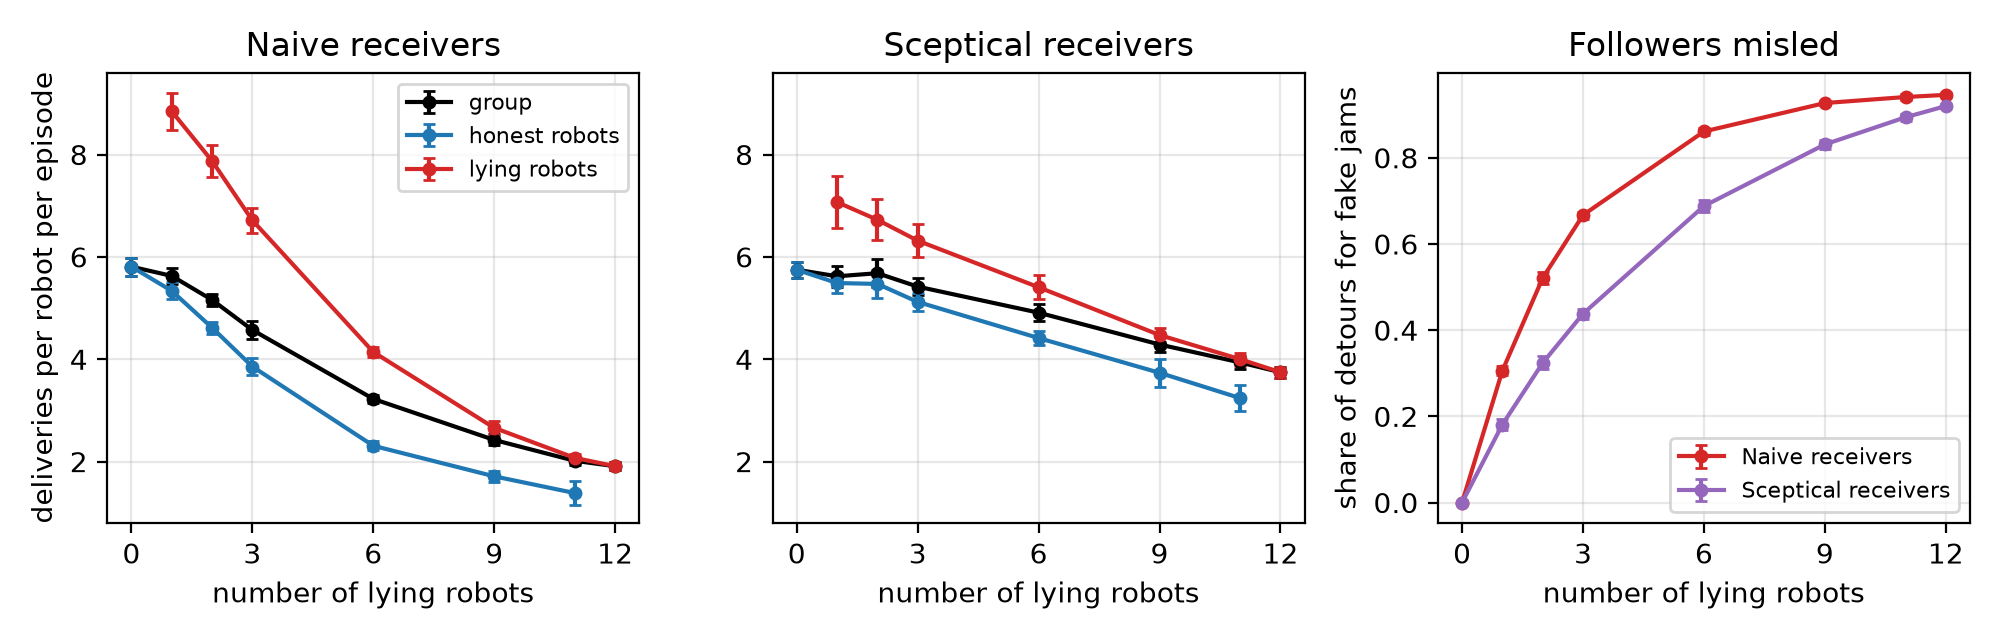
\includegraphics[width=\textwidth]{figures/fake_jams_hype_compare.png}
  \caption{Lying harms the group in the congestion setting. The first $k$ of 12 robots post fake jams and the rest report real jams, with fixed policies and no credit (10 batches of 20 episodes, 95\% CIs). Left and middle: deliveries per robot per episode for the group, the honest robots and the lying robots, with naive and with sceptical receivers. Right: share of detours that were for fake jams.}
  \label{fig:hype}
\end{figure*}

\paragraph{\tvc{} removes lying and raises throughput.}
\Cref{tab:pogema} gives the lifelong comparison at $\lambda=0$. Without credit, selfish robots post a fake jam on 99.2\% of their opportunities and report 44.7\% of the real jams elsewhere. Popularity credit leaves the lie rate at 99.9\% and raises useful reports to 94.6\%, but throughput falls from 0.080 to 0.037, as in the hype sweep, where throughput falls as more robots lie (\cref{fig:hype}). \tvc{} cuts the lie rate to 0.2\%, raises useful reports to 98.8\%, and raises throughput to 0.266, 3.3 times that of no credit and 7.2 times that of popularity credit.
% Ratios below are from logs/fake_jams_envs.md (3-decimal rounding), so they are approximate.
The other designs fall between these. Reputation alone, that is sceptical receivers with no credit, keeps the lie rate at 80.1\% and reaches only about 1.5 times the throughput of no credit. Accuracy credit removes lying (0.1\%) by silencing the robots, with 1.2\% useful reports, and its throughput is below that of no credit (about 0.75 times). A shared return with $\lambda=(N-1)/N$ is the closest competitor: it cuts lying to 6.3\% and reaches about 3.1 times the throughput of no credit, but it needs every robot to weigh the others' deliveries as much as its own, which \tvc{} does not.

% POGEMA lifelong MAPF, lambda = 0, 10 seeds (source: logs/fake_jams_pogema.md).
% ICML: table captions go ABOVE the table.
\begin{table}[t]
  \caption{POGEMA lifelong MAPF ($\lambda=0$, 10 seeds, mean $\pm$ 95\% CI). Lie rate is the percentage of opportunities on which a robot posts a fake jam on its own route, useful is the percentage of real jams elsewhere that it reports, and throughput is POGEMA's \texttt{avg\_throughput}, the deliveries per step summed over the 12 robots.}
  \label{tab:pogema}
  \centering
  \small
  \setlength{\tabcolsep}{3pt}
  \begin{tabular}{lccc}
    \toprule
    Rule & Lie rate (\%)  & Useful (\%)  & Throughput  \\
    \midrule
    None       & $99.2 \pm 0.0$ & $44.7 \pm 1.5$ & $0.080 \pm 0.002$ \\
    Popularity & $99.9 \pm 0.0$ & $94.6 \pm 0.8$ & $0.037 \pm 0.001$ \\
    \textbf{TVC} & $\mathbf{0.2 \pm 0.1}$ & $\mathbf{98.8 \pm 0.7}$ & $\mathbf{0.266 \pm 0.007}$ \\
    \bottomrule
  \end{tabular}
\end{table}


\paragraph{\tvc{} holds at every prosocial weight.}
Across the prosocial weight $\lambda$ (\cref{fig:lam}), popularity credit keeps the lie rate at 99.8--99.9\% and throughput at 0.003, and \tvc{} holds the lie rate at 0.2\% or less at every $\lambda$, with throughput 0.022--0.023. With no credit, lying is 99.2\% at $\lambda=0$ and still 91.9\% at $\lambda=0.75$, and falls to 2.5\% only at $\lambda=1$, where throughput rises to 0.021. This agrees with the calibrated threshold, $\lambda\approx0.93$, below which a lie is profitable without credit.

\begin{figure}[t]
  \centering
  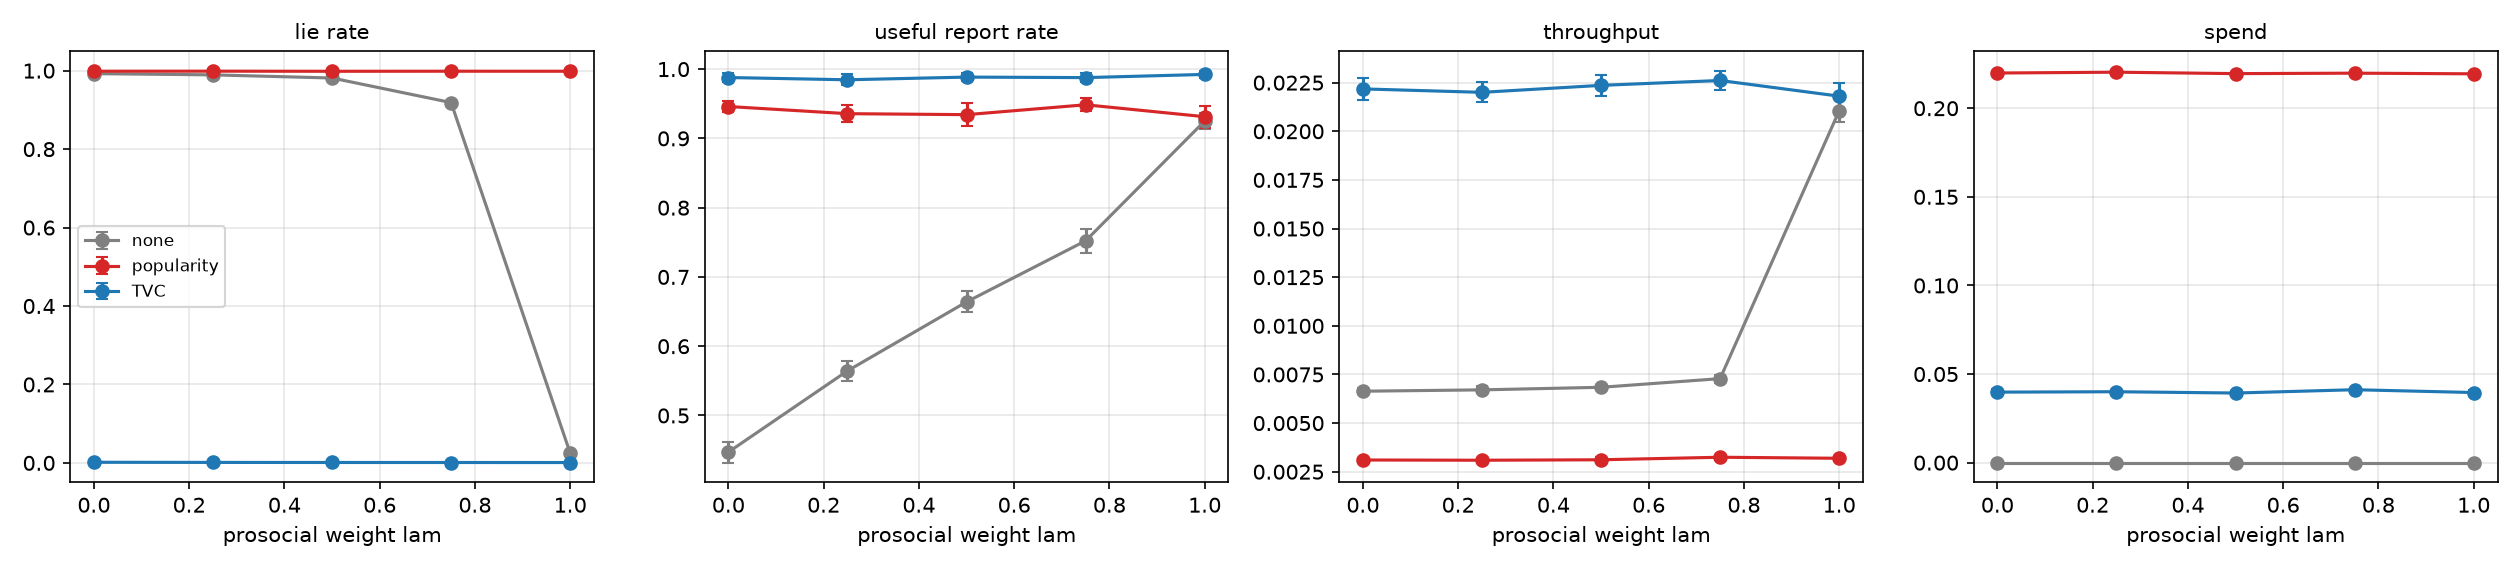
\includegraphics[width=\linewidth]{figures/fake_jams_lam.png}
  \caption{Learned behaviour by credit rule and prosocial weight $\lambda$ (10 seeds, 95\% CIs).}
  \label{fig:lam}
\end{figure}

% \paragraph{The fine follows the theory.}
% The fine sweep (\cref{fig:fine}, $\lambda=0$) brackets the calibrated threshold $\philo=2.25$. Lying is 99.3\% with no fine and 98.3\% at $0.5\philo$, falls to 62.4\% at $\philo$ and to 0.9\% at $2\philo$, so it collapses between $\philo$ and $2\philo$, within a factor of two of the theory. \Cref{app:ablation} also shows that removing the audits or the fine brings lying back, that the bonus is not needed in this setting, and that \tvc{} raises throughput only when receivers act on claims.

% \begin{figure}[t]
%   \centering
%   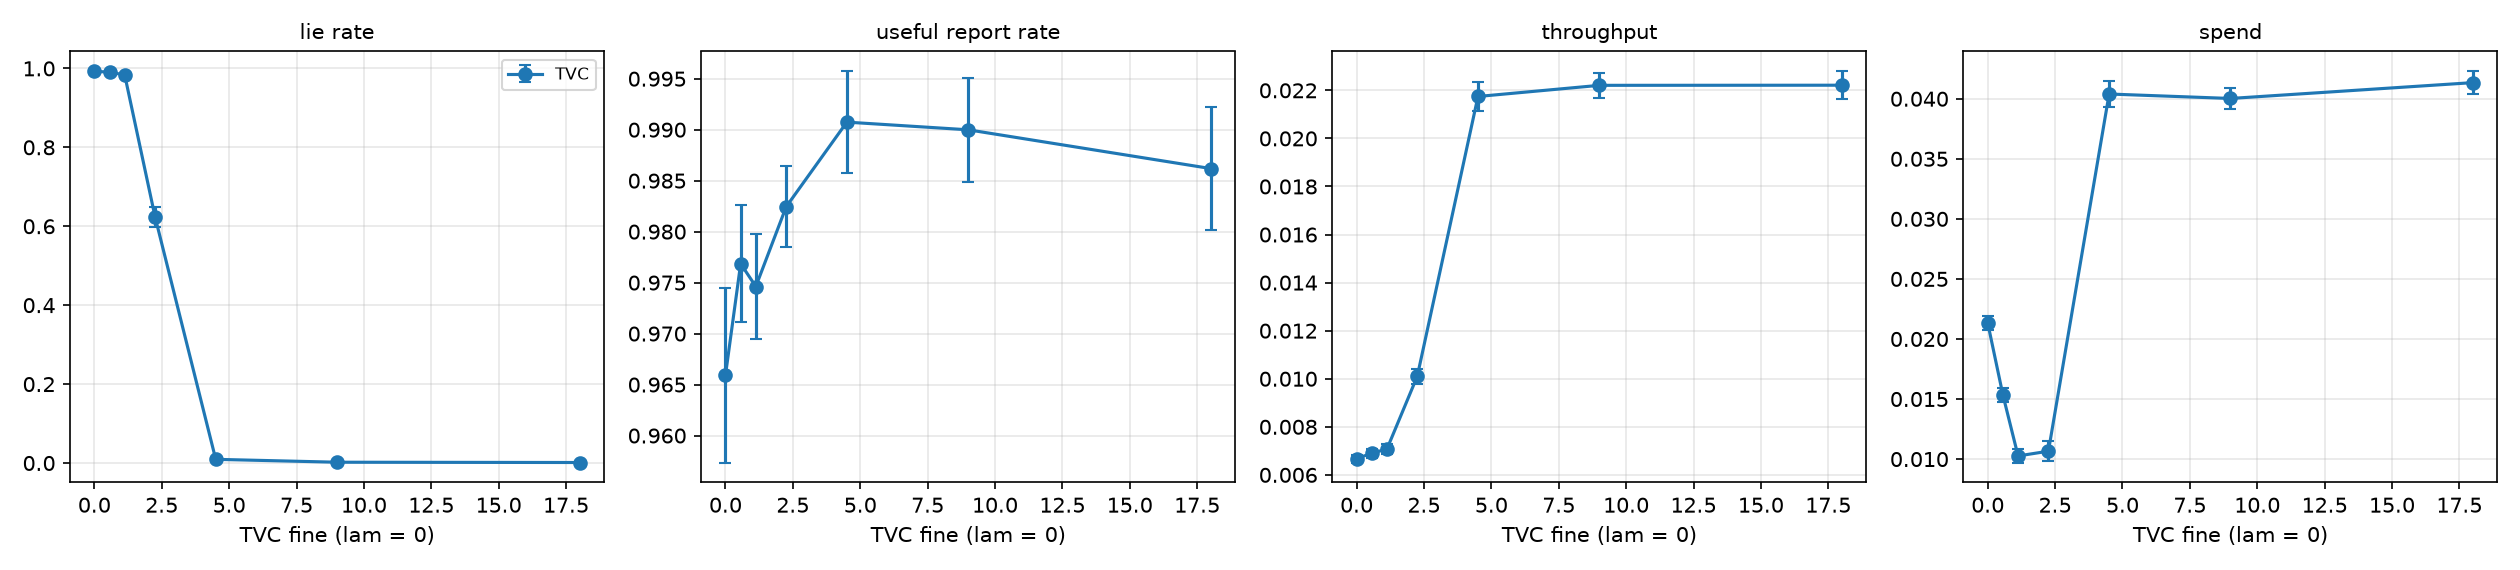
\includegraphics[width=\linewidth]{figures/fake_jams_fine.png}
%   \caption{TVC fine sweep at $\lambda=0$. Lying collapses between $\philo$ and $2\philo$ (10 seeds, 95\% CIs).}
%   \label{fig:fine}
% \end{figure}

% \todo{Scaling (agents, map size).}

\FloatBarrier
\section{Conclusion}
\label{sec:conclusion}

\paragraph{Conclusion.}
Credit that rewards agents for being relied on rewards attention, not accuracy, and learning agents respond by exaggerating. We proposed truthful verified credit (\tvc{}), which gives credit only for verified value, adds a bonus for every checked claim, and fines audited false claims. The fine needed to outweigh a lie's outside gain grows as $1/p$ in the audit rate $p$. Across both experiments, \tvc{} nearly eliminates exaggeration and keeps agents reporting. Its welfare is comparable to popularity credit when receivers can decode exaggeration cheaply, and well above both baselines when receivers act on claims. Lying stays low at every prosocial weight and collapses close to the theoretical fine threshold. \tvc{} is called for when credit follows reliance, lying is profitable outside the credit, lying harms others, and a sample of claims can be audited. When agents weigh the others' payoffs almost as much as their own, a shared return alone comes close.

\paragraph{Limitations.}
\tvc{} elicits truth, not usefulness. In the bandit its welfare matches popularity credit but does not exceed it, because calibrated receivers decode exaggeration cheaply, and designs that raise exploration reach higher welfare without making reports honest. The fine rule is derived for a sender that maximises expected reward in a single round. It also assumes that checks reveal the truth exactly, that audits are independent, and that receivers never follow a claim that cannot help them. Our testbeds are simulated, and the outside gain of a lie is calibrated from short runs, not an emergent property. The bonus accounts for most of the credit given in the congestion setting, yet removing it changes little there. Future work includes noisy verification, the cost of audits, and fleets with real data.


% Acknowledgements should only appear in the accepted version.
% \section*{Acknowledgements}

\section*{Impact Statement}
% REQUIRED by ICML: unnumbered, before the references; does not count toward the page limit.
This paper studies incentive design for learning agents that share information.
Mechanisms that reward truthful, verified reports could make multi-agent systems more reliable and could reduce manipulation of shared information channels.
The same tools could be misused to design audits that are unfair to some agents, and our design assumes accurate audits; deployments should account for audit errors.
Beyond these points, we see no societal consequences that must be specifically highlighted here.

\bibliography{references}
\bibliographystyle{icml2026}

%%%%%%%%%%%%%%%%%%%%%%%%%%%%%%%%%%%%%%%%%%%%%%%%%%%%%%%%%%%%%%%%%%%%%%%%%%%%%%%
% APPENDIX (same PDF; not counted toward the 8-page limit)
%%%%%%%%%%%%%%%%%%%%%%%%%%%%%%%%%%%%%%%%%%%%%%%%%%%%%%%%%%%%%%%%%%%%%%%%%%%%%%%
\newpage
\appendix
\onecolumn
\section{Analysis of Truthful Reporting in MAB with private payoff}
\label{app:analysis_mab}

\begin{proposition}[Truthful reporting is interim strictly dominant in one round]
  \label{prop:dominance}
  In one round, truthful reporting is a interim strictly dominant strategy for the sender \cref{eq:reward} if $p\,(\eta+\varphi) > \eta\,\sbar+\Gamma$ and $p\eta>\xi$.

\end{proposition}

\begin{proof}
  Let us reconsider the problem introduced in \cref{sec:problem}. We relax the problem into a single round with one sender. Thus, for brevity, we will drop the "$t$" notation. In this case, a \emph{sender} $i$ found an arm, and choose to make an report $m\in\{\varnothing\}\cup\mathbb R_{>0}$. A report $m$ is truthful if $m=\theta$ and untruthful otherwise, whether exaggerated ($m>\theta$) or understated ($m<\theta$), and $m=\varnothing$ is silence. Everyone else, receivers and other senders, is collapsed into an arbitrary \emph{opponent profile}, denoted $\sigma_{-i}$: any map from the posted claim to a distribution over their actions.

We assume the follows.

\begin{enumerate}[label=A\arabic*]
  \item \emph{Separability.} Given the action profile, $u_i$ does not depend on $m_i$. Claims affect $i$'s reward only through $C_i$ and through receivers' future behaviour.
  \item \emph{Unforgeable verification.} On checked claims the designer learns $\theta_i$ exactly, and followers cannot misreport it.
  \item \emph{Independent audits.} $a_i$ is independent of $(m, d, h)$.
  \item \emph{Untruthful reports are detected.} Every untruthful report, whether exaggerated or understated, misses the tolerance: $m\neq\theta \Rightarrow |m/\theta-1|>\tau$.
  \item \emph{Truthful reports do not hurt the sender.} A truthful report does not lower the sender's weighted payoff $(1-\lambda)u_i+\lambda\bar u_{-i}$ relative to silence. This holds when receivers never follow a truthful claim at a loss to themselves and following does not change the sender's own payoff.
\end{enumerate}

\begin{table}[t]
  \caption{Reward $r$ of a sender $i$ under \tvc{} in one round, based on \cref{eq:reward}, in units of $\vbar$. Each row is what happens to the claim: whether some receiver follows it and whether the random audit checks it. Each column is what the sender does: report truthfully ($m=\theta$), report untruthfully ($m\neq\theta$, exaggerated or understated) or stay silent ($m=\varnothing$). Each cell is \cref{eq:reward} evaluated with the credit of \cref{eq:tvc} for the case in its row and column, with $S=S(m,\theta)$. Every claim bears the posting cost $\xi$. An untruthful report never passes the verification gate, so it earns no gain credit, and it gains the outside gain $\Gamma$ only when it is followed, because only then do believers act on it. We take the outside effect of a truthful claim as zero, since a positive effect only favours truth. Silence posts no claim, so it bears no cost and earns $0$.}
  \label{tab:cases}
  \centering
  \small
  \setlength{\textwidth}{3pt}
  \begin{tabular}{lccc}
    \toprule
    Case & Truth & Untruthful & Silence \\
    \midrule
    Followed, audited         & $\min(g,\Bbar)+\eta-\xi$ & $\Gamma+\eta S-\varphi-\xi$ & $0$ \\
    Followed, not audited     & $\min(g,\Bbar)+\eta-\xi$ & $\Gamma+\eta S-\xi$         & $0$ \\
    Not followed, audited     & $\eta-\xi$               & $\eta S-\varphi-\xi$        & $0$ \\
    Not followed, not audited & $-\xi$                   & $-\xi$                      & $0$ \\
    \bottomrule
  \end{tabular}
\end{table}

\cref{tab:cases} shows the reward $r_i$ of a sender under \tvc{} in one round.

Fix any opponent profile $\sigma_{-i}$, and write $O(m)$ for the expected value of $(1-\lambda)u_i+\lambda\bar u_{-i}$ when the sender reports $m$. By separability (A1), $O(m)$ depends on $m$ only through how the opponents respond, so $O(m)\le O(\theta)+\Gamma$ for every untruthful report $m$, and $O(\theta)\ge O(\varnothing)$ by A5. The audit is independent of the claim and the receivers (A3), so a non-silent claim is checked with probability at least $p$, and a report that fails the gate is fined with probability exactly $p$. By \emph{interim strict dominance} we mean that, for every true value $\theta$ and every opponent profile $\sigma_{-i}$, the expected reward of truthful reporting exceeds that of every other report. The sender knows its own find $\theta$ when it reports, but not yet the audit draw or the receivers' response, and the expectation is over those two. It does not require truth to be best in every realisation, and it is not (silence is better in the last row of \cref{tab:cases}). Write $\bar r(m)$ for the expected reward of report $m$.

A truthful claim passes the gate and its gain credit is nonnegative. It earns the bonus $\eta$ whenever it is checked, which happens with probability at least $p$. So, whatever the receivers do,
\[
  \bar r(\theta)\;\ge\;O(\theta)-\xi+p\eta .
\]

By A4 an untruthful report fails the gate, so it earns no gain credit and is fined $\varphi$ when audited. Its bonus is at most $\eta\sbar$, because its score is at most $\sbar$ and it is checked at most always. So, whatever the receivers do,
\[
  \bar r(m)\;\le\;O(\theta)+\Gamma-\xi+\eta\sbar-p\varphi .
\]

Silence bears no cost and cannot be followed or audited, so $\bar r(\varnothing)=O(\varnothing)\le O(\theta)$.

Subtracting, for every value $\theta$, every untruthful report $m\neq\theta$ and every $\sigma_{-i}$,
\[
  \bar r(\theta)-\bar r(m)\;\ge\;p(\eta+\varphi)-\eta\sbar-\Gamma\;>\;0
  \qquad\text{and}\qquad
  \bar r(\theta)-\bar r(\varnothing)\;\ge\;p\eta-\xi\;>\;0,
\]
both by the conditions of \cref{prop:dominance}. Neither bound depends on $m$ or on $\sigma_{-i}$, so truthful reporting is interim strictly dominant. 
\end{proof}



% \subsection{From One Round to All Rounds}
% \label{app:allrounds}
% The game lasts $T$ rounds, strategies may depend on the history, and the sender maximises its expected discounted reward $R=\sum_{t=1}^{T}\gamma^{t-1}r^t$ with $\gamma\in(0,1]$. In every round in which the sender has a find, it reports $m^t$, and the audit draw $a^t$ is independent of everything before round $t$ and of $m^t$. We assume that the conditions of \cref{prop:dominance} and A1--A5 hold in every round, and add one assumption.

% \begin{enumerate}[label=A\arabic*, start=6]
% \item \emph{A report has no effect on the future.} What the sender reports in a round changes its reward in that round only. It does not change the sender's own state, how receivers treat it later, or the audits. Effects that last while followers stay committed are already counted in that round's reward, in the credit and in $O(m^t)$.
% \end{enumerate}

% \begin{proposition}[All rounds]
%   \label{prop:allrounds}
%   Under A1--A6, the strategy that reports truthfully in every round strictly dominates every other strategy, up to strategies that differ from it only at histories that occur with probability zero.
% \end{proposition}

% \textbf{Proof.} Fix any opponent strategy $\sigma_{-i}$, which may depend on the history. Let $V^t(h)$ be the largest expected discounted reward that the sender can obtain from round $t$ on after history $h$, with $V^{T+1}=0$. Then
% \[
%   V^t(h)=\max_{m}\Big\{\bar r^t(m\mid h)+\gamma\,\mathbb E\big[V^{t+1}(h')\mid h,m\big]\Big\},
% \]
% where $\bar r^t(m\mid h)$ is the expected round-$t$ reward of report $m$. By the one-round proof, $\bar r^t(\theta\mid h)-\bar r^t(m\mid h)\ge\delta>0$ for every report $m\neq\theta$, whatever the receivers do in round $t$. By A6 the continuation term is the same for every $m$. So the bracket at $m=\theta$ exceeds the bracket at any other $m$ by at least $\delta$, and truth is the unique maximiser at every history of every round. Hence the all-truthful strategy is a best response to $\sigma_{-i}$, and a strategy that deviates at a history $h^t$ reached with probability $\Pr(h^t)$ loses at least $\gamma^{t-1}\Pr(h^t)\,\delta>0$ against it. Since $\sigma_{-i}$ was arbitrary, truthful reporting in every round is strictly dominant, and strategies that differ from it only at histories of probability zero have the same expected reward. \qed

% \textbf{Learning receivers.} A6 fails when receivers learn from checks, as the sceptical and calibrated receivers in our experiments do, because a report then changes their later rules. The proof still goes through under a weaker assumption, which makes the continuation term largest at $m=\theta$ instead of equal for all $m$:
% \begin{enumerate}[label=A\arabic*, start=7]
%   \item \emph{ (a lie never helps later)}: after a truthful report, the sender's expected later reward is at least as high as after any other report. A6 is the case where they are equal.
% \end{enumerate}

%   A7 is natural, since a lie that is checked lowers the receivers' trust, an unchecked lie leaves it unchanged, and a truthful claim does not lower it, but we have not proved it for every learning rule.

\section{Sizing the Fine}
\label{app:fine}


We size the fine against the outside gain $\Gamma$ of a lie (\cref{eq:gamma}) and the posting cost $\xi$ in the reward \cref{eq:reward}.

By the analysis above, truth earns at least $p\eta\vbar$ from the credit, and a lie earns at most $(\eta\sbar-p\varphi)\vbar$ from the credit plus $\Gamma$ outside it. Both bear the posting cost $\xi$, which cancels. Truth stays strictly better than a lie when $p\eta>\eta\sbar-p\varphi+\Gamma$, which gives
\begin{equation}
  \varphi>\philo = \frac{\eta\,\sbar+\Gamma}{p}-\eta .
  \label{eq:fine}
\end{equation}
A larger outside gain needs a larger fine, and fewer audits (a smaller $p$) need a larger fine too, in proportion to $1/p$. If lies score almost nothing ($\sbar\approx0$), the condition reads $\varphi>\Gamma/p-\eta$. Against silence, a truthful claim earns at least $p\eta\vbar$ of credit and bears the posting cost, so truth beats silence when $p\eta\vbar>\xi$, assuming a truthful claim has no negative outside effect. When the sender has no truthful claim to make, as at a free doorway in the congestion setting, its alternative to a lie is silence, which bears no posting cost, so $\xi$ does not cancel. A lie then beats silence unless $\varphi>(\eta\sbar+\Gamma-\xi)/p$, which is $(\Gamma-\xi)/p$ when $\sbar\approx0$. In the congestion experiment, $\philo$ denotes this threshold.


% \paragraph{Each part is needed.}
% Each part of \tvc{} closes a row of \cref{tab:cases} that the other two leave open, and removing it brings back a failure of reliance credit.

% \paragraph{Verified externality credit stops the hype.}
% Without the gate $V_i^t$, a followed liar collects the followers' gain like a true claim, so the liar's best case rises by up to $\Bbar$ and the fine has to outbid whatever the lie can attract; exaggeration is rewarded as it is under popularity credit. The gate removes that term at no cost to truth, because a truthful claim passes it. It is also the only part of the credit that rises with how much a find helps others; without it, credit would depend on accuracy alone.

% \paragraph{The checked score bonus stops silence.}
% Without the bonus ($\eta=0$), the fine still makes truth beat a lie by $p\varphi$, but an unfollowed true claim earns $0$, the same as silence. A low-value find is then not worth reporting once reporting costs anything, and no one reports because no one follows, which is the incentive behind the file drawer. The bonus is given on any checked claim, so a true claim is worth at least $p\eta$ even when nobody follows it.

% \paragraph{Audits and the lying cost stop outside gain.}
% Without audits ($p=0$), an unfollowed claim is never checked, so truth, any lie and silence all earn $0$, and the bonus cannot reach ignored claims. Without the fine ($\varphi=0$), a lie's best case is $\eta\sbar+\Gamma$ against truth's worst case $p\eta$, so truth wins only if $\Gamma<\eta(p-\sbar)$: the audit rate must exceed the best lie's score, and any larger outside gain goes unpunished. The fine is the only part that scales with the temptation, and it can be large while audits stay rare because its size grows as $1/p$ ( see \cref{eq:fine}).

% The ablations in \cref{sec:experiments} remove each part in turn.

\section{Notation}
\label{app:notation}

\Cref{tab:notation} lists the symbols used in the paper. Amounts of credit are in units of the mean arm value $\vbar$.

\begin{table}[t]
  \caption{Notation.}
  \label{tab:notation}
  \centering
  \small
  \begin{tabular}{p{0.13\linewidth}p{0.77\linewidth}}
    \toprule
    Symbol & Meaning \\
    \midrule
    \multicolumn{2}{l}{\emph{Environment}} \\
    $N$, $K$, $T$ & number of agents, arms and rounds \\
    $v_k$, $F$, $\vbar$ & value of arm $k$, its distribution, and the mean value (unit of credit) \\
    $\mathcal K_i^t$, $b_i^t$ & arms known to agent $i$ and the value of its best known arm \\
    $c$ & cost of exploring an unknown arm \\
    $u_i^t$, $\pi_i$ & own payoff of agent $i$ and its policy \\
    $y_i^t$, $\epsilon_i^t$, $\sigma$ & noisy observation $y_i^t=v_ke^{\epsilon_i^t}$, its noise, and the noise level \\
    $\theta_i^t$ & true value of the arm that $i$ reports on \\
    \midrule
    \multicolumn{2}{l}{\emph{Claims and reliance}} \\
    $m_i^t$, $\varnothing$ & claim of sender $i$ and silence \\
    $\kappa_i^t$ & inflation factor $m_i^t/y_i^t$ ($1$ means truthful) \\
    $d_j^t$, $\rho_j$, $h_j^t$ & whom receiver $j$ follows, its receiver rule, and its history \\
    $L$ & number of rounds a follower stays committed \\
    $g_{ji}^t$ & gain of follower $j$ from $i$'s claim, $L(\theta_i^t-b_j^t)^+$ \\
    $\mathcal F_i^t$, $f_i^t$ & follow set $\{j:d_j^t=i\}$ and the indicator that it is non-empty \\
    \midrule
    \multicolumn{2}{l}{\emph{\tvc{}}} \\
    $\tau$ & tolerance for verification \\
    $V_i^t$ & verification gate, $\mathbb 1[|m_i^t/\theta_i^t-1|\le\tau]$ \\
    $\Bbar$ & cap on gain credit per follower (in units of $\vbar$) \\
    $\eta$, $w$ & bonus weight and score width \\
    $S(m,\theta)$, $\sbar$ & score of a claim and the best score of any claim outside the tolerance \\
    $a_i^t$, $p$ & random audit and its probability \\
    $\chi_i^t$ & claim is checked (audited or followed) \\
    $\varphi$, $\philo$ & fine for an audited false claim and the smallest fine that keeps truth dominant \\
    $C_i^t$ & \tvc{} credit to sender $i$ \\
    \midrule
    \multicolumn{2}{l}{\emph{Outside gain}} \\
    $\lambda$ & prosocial weight on the others' mean payoff in the reward ($0$ selfish, $1$ fully cooperative) \\
    $r_i^t$, $\bar u_{-i}^t$ & total reward of sender $i$ and the mean payoff of the other agents \\
    $G_1$, $D_1$ & liar's gain and damage to the others from one lie \\
    $\xi$ & cost of posting a claim \\
    $\Gamma$ & outside gain of a lie over a truthful claim, $(1-\lambda)G_1-\lambda D_1$ \\
    $\Delta$ & margin by which truth beats a lie, $p(\eta+\varphi)-\eta\sbar$ \\
    \bottomrule
  \end{tabular}
\end{table}

\section{Experimental Details}
\label{app:details}

\subsection{Hyperparameters}

\Cref{tab:hyper-bandit,tab:hyper-jams} list every setting of the two experiments. Credit amounts are in units of the mean arm value $\vbar$ in the bandit, and in deliveries in the congestion setting.

\begin{table}[t]
  \caption{Multi-agent bandit settings.}
  \label{tab:hyper-bandit}
  \centering
  \small
  \begin{tabular}{p{0.52\linewidth}p{0.38\linewidth}}
    \toprule
    Setting & Value \\
    \midrule
    Agents $N$, arms $K$, rounds $T$ & $10$, $50$, $100$ \\
    Episodes, independent runs & $1000$, $32$ \\
    Exploration cost $c$ & $0.5\vbar$ \\
    Commitment $L$ & $3$ rounds \\
    REINFORCE learning rate, discount & $0.1$, $0.9$ \\
    Baseline step size & $0.05$ \\
    Calibrated receivers' learning rate & $0.3$ \\
    Popularity credit & $2\vbar$ per follower \\
    Accuracy credit & $1\times$ follower's signed gain \\
    Keeping-exploring credit & $3\vbar$ per exploration \\
    \tvc{}: $\tau$, $\Bbar$, $\eta$, $w$, $p$, $\varphi$ & $0.05$, $8$, $2$, $0.05$, $0.2$, $8$ \\
    \bottomrule
  \end{tabular}
\end{table}

\begin{table}[t]
  \caption{MAPF fake-jam settings.}
  \label{tab:hyper-jams}
  \centering
  \small
  \begin{tabular}{p{0.52\linewidth}p{0.38\linewidth}}
    \toprule
    Setting & Value \\
    \midrule
    Robots $N$, observation radius, steps & $12$, $3$, $256$ \\
    Episodes, seeds & $150$, $10$ \\
    Jam radius, jam queue & $2$ steps, $3$ robots \\
    Avoidance duration, claim lifetime & $20$, $20$ steps \\
    Sceptical receivers' learning rate & $0.3$ \\
    Cost of posting a claim $\xi$ & $0.05$ \\
    Prosocial weight $\lambda$ & $0$ (main), swept in $\{0,\dots,1\}$ \\
    REINFORCE learning rate & $0.1$ \\
    Baseline step size, advantage clip & $0.05$, $[-10,10]$ \\
    Popularity credit & $1$ per believer \\
    Accuracy credit & $1\times$ steps saved \\
    \tvc{}: $\tau$, $\Bbar$, $\eta$, $p$, $\varphi$ & $0.05$, $8$, $2$, $0.2$, $15$ \\
    \bottomrule
  \end{tabular}
\end{table}

\subsection{Calibrating the Temptation}

The congestion setting needs the per-believer gain, harm and benefit of a claim, which enter the sender's learning signal (\cref{eq:reward}). We measure them before training, once for each layout, with no credit and with hand-set claim policies on common random seeds, $30$ episodes each. In every policy only robot~$0$ is the sender and the other robots stay silent, except in the last. The \emph{silent} policy never posts. The \emph{reporter} posts true jams elsewhere, and the \emph{liar} posts fake jams on its own route. In \emph{all-liars} every robot posts fake jams on its own route. Writing $T_\bullet$ for the mean deliveries per robot under policy $\bullet$ and $b_\bullet$ for the number of believers of the sender's claims,
\begin{align*}
  \text{own gain} &= \frac{T_{\text{liar}}^{(0)}-T_{\text{silent}}^{(0)}}{b_{\text{liar}}}, &
  \text{benefit} &= \frac{\bar T_{\text{reporter}}^{(-0)}-\bar T_{\text{silent}}^{(-0)}}{b_{\text{reporter}}},
\end{align*}
\[
  \text{harm}=\frac{N\,(\bar T_{\text{silent}}-\bar T_{\text{all-liars}})+\text{own gain}\cdot b_{\text{all-liars}}}{(N-1)\,b_{\text{all-liars}}},
\]
where $(0)$ is robot~$0$ and $(-0)$ the mean of the other robots. We measure the harm with all robots lying because a single liar among silent robots barely hurts: traffic spreads out. These per-believer values give $\Gamma$ in \cref{eq:gamma}, and from it the fine threshold $\philo$ in \cref{eq:fine} with $\sbar\approx0$.

\subsection{Seeds, Statistics and Compute}

In the bandit, the $32$ runs are independent policies and arm values simulated as one batch from one random generator (seed $0$). The confidence interval is $1.96\,s/\sqrt{32}$, where $s$ is the standard deviation of the per-run mean over the last $100$ episodes. In the congestion setting, each seed trains from scratch, the metric of a seed is its mean over the last $50$ of $150$ episodes, and the confidence interval is the $t$-interval over seeds. All runs use the CPU only (an Apple M4 Max with 14 cores and 36\,GB of memory), with seeds and variants distributed over a process pool.


% \subsection{Learning Curves}
% \label{app:curves}

% Agents learn online, so we report the mean over the last 100 of 1000 episodes (\cref{sec:experiments}). \Cref{fig:curves-naive,fig:curves-calibrated} show the full learning curves of the bandit experiment for every credit design.

% \begin{figure*}[t]
%   \centering
%   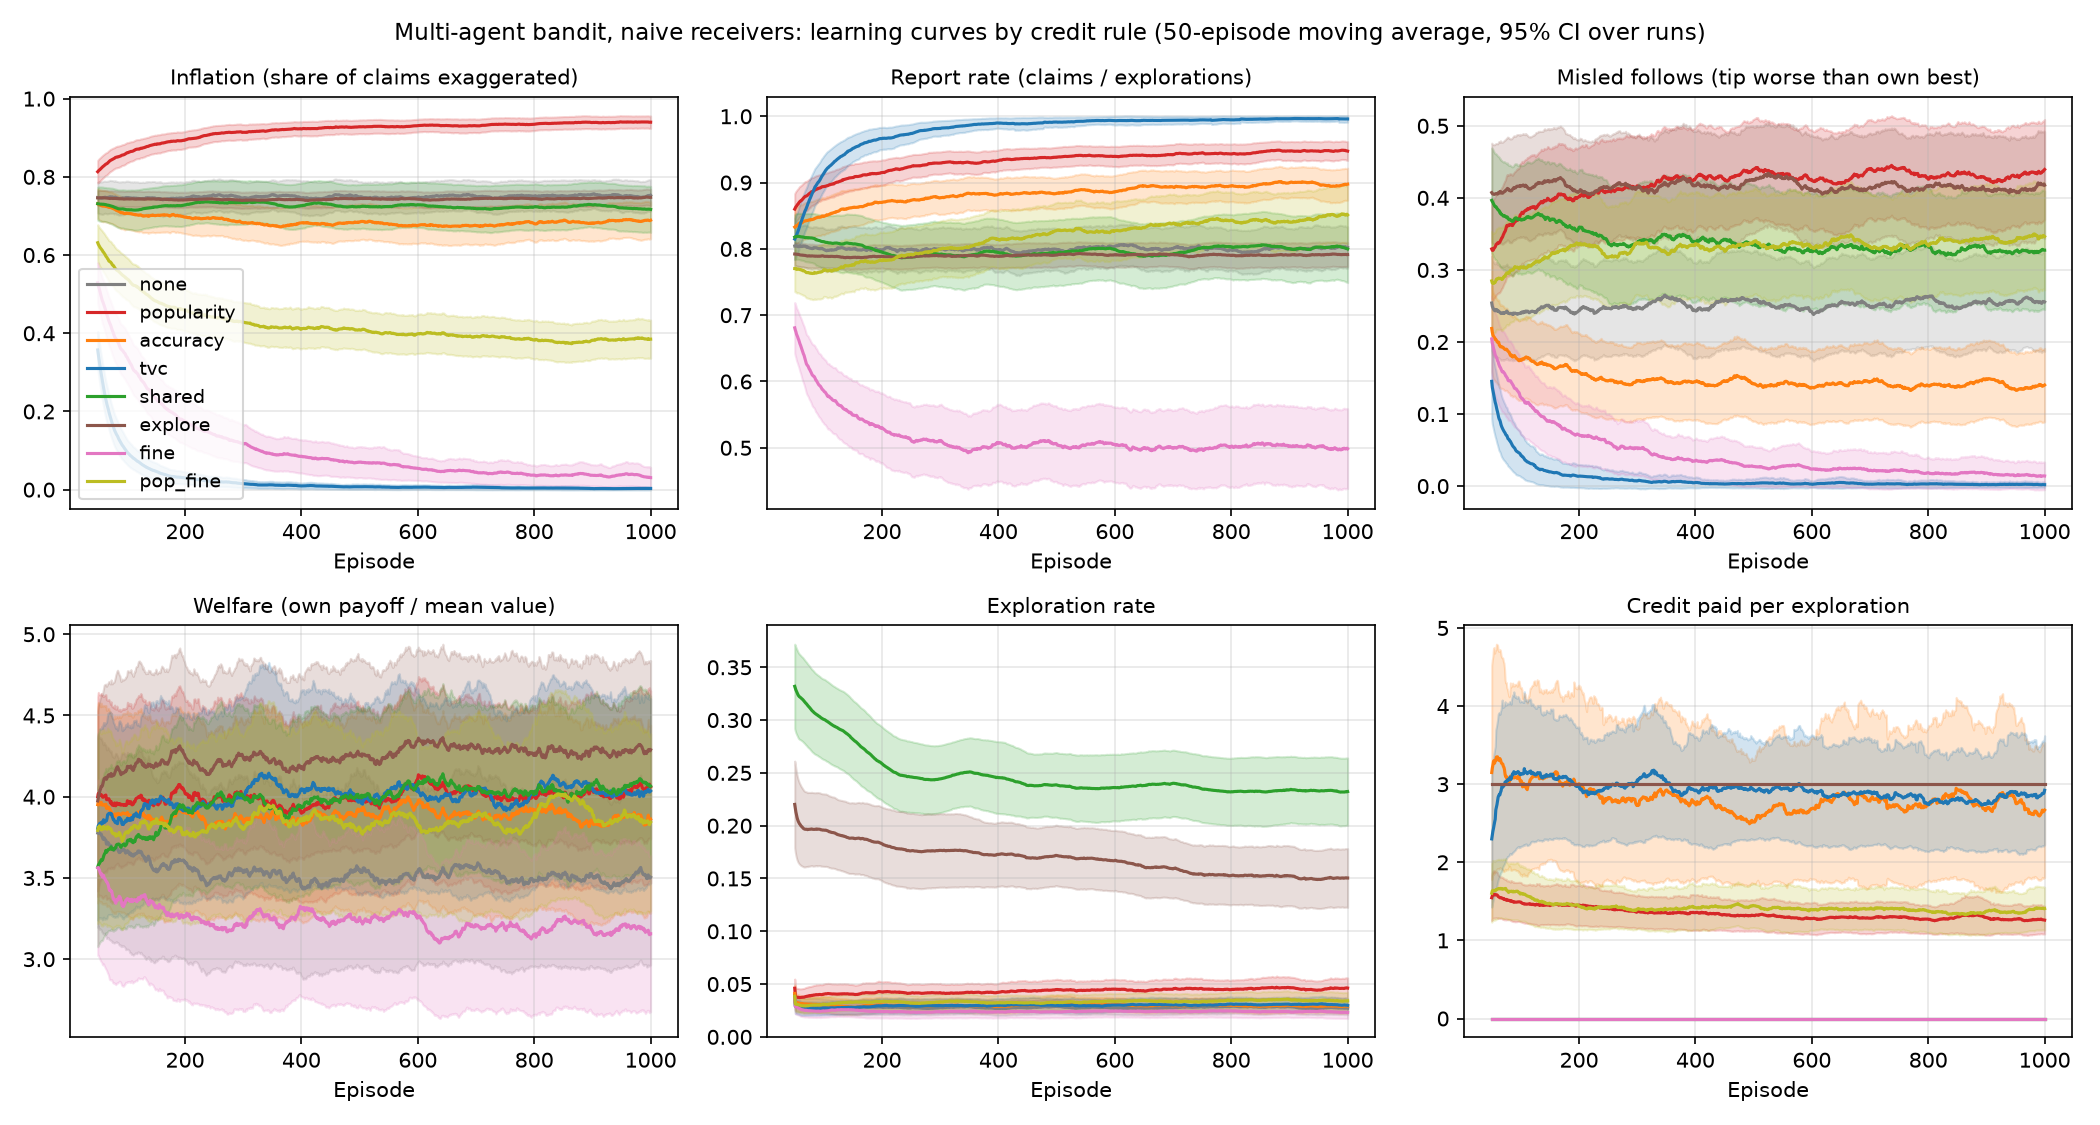
\includegraphics[width=\textwidth]{figures/bandit_naive.png}
%   \caption{Learning curves in the multi-agent bandit with naive receivers (50-episode moving average, 95\% confidence interval over 32 runs). Each panel is one metric and each line one credit design. \tvc{}'s inflation and misled follows settle near zero within about 300 episodes, popularity credit settles at high inflation, and welfare intervals overlap for most designs.}
%   \label{fig:curves-naive}
% \end{figure*}

% \begin{figure*}[t]
%   \centering
%   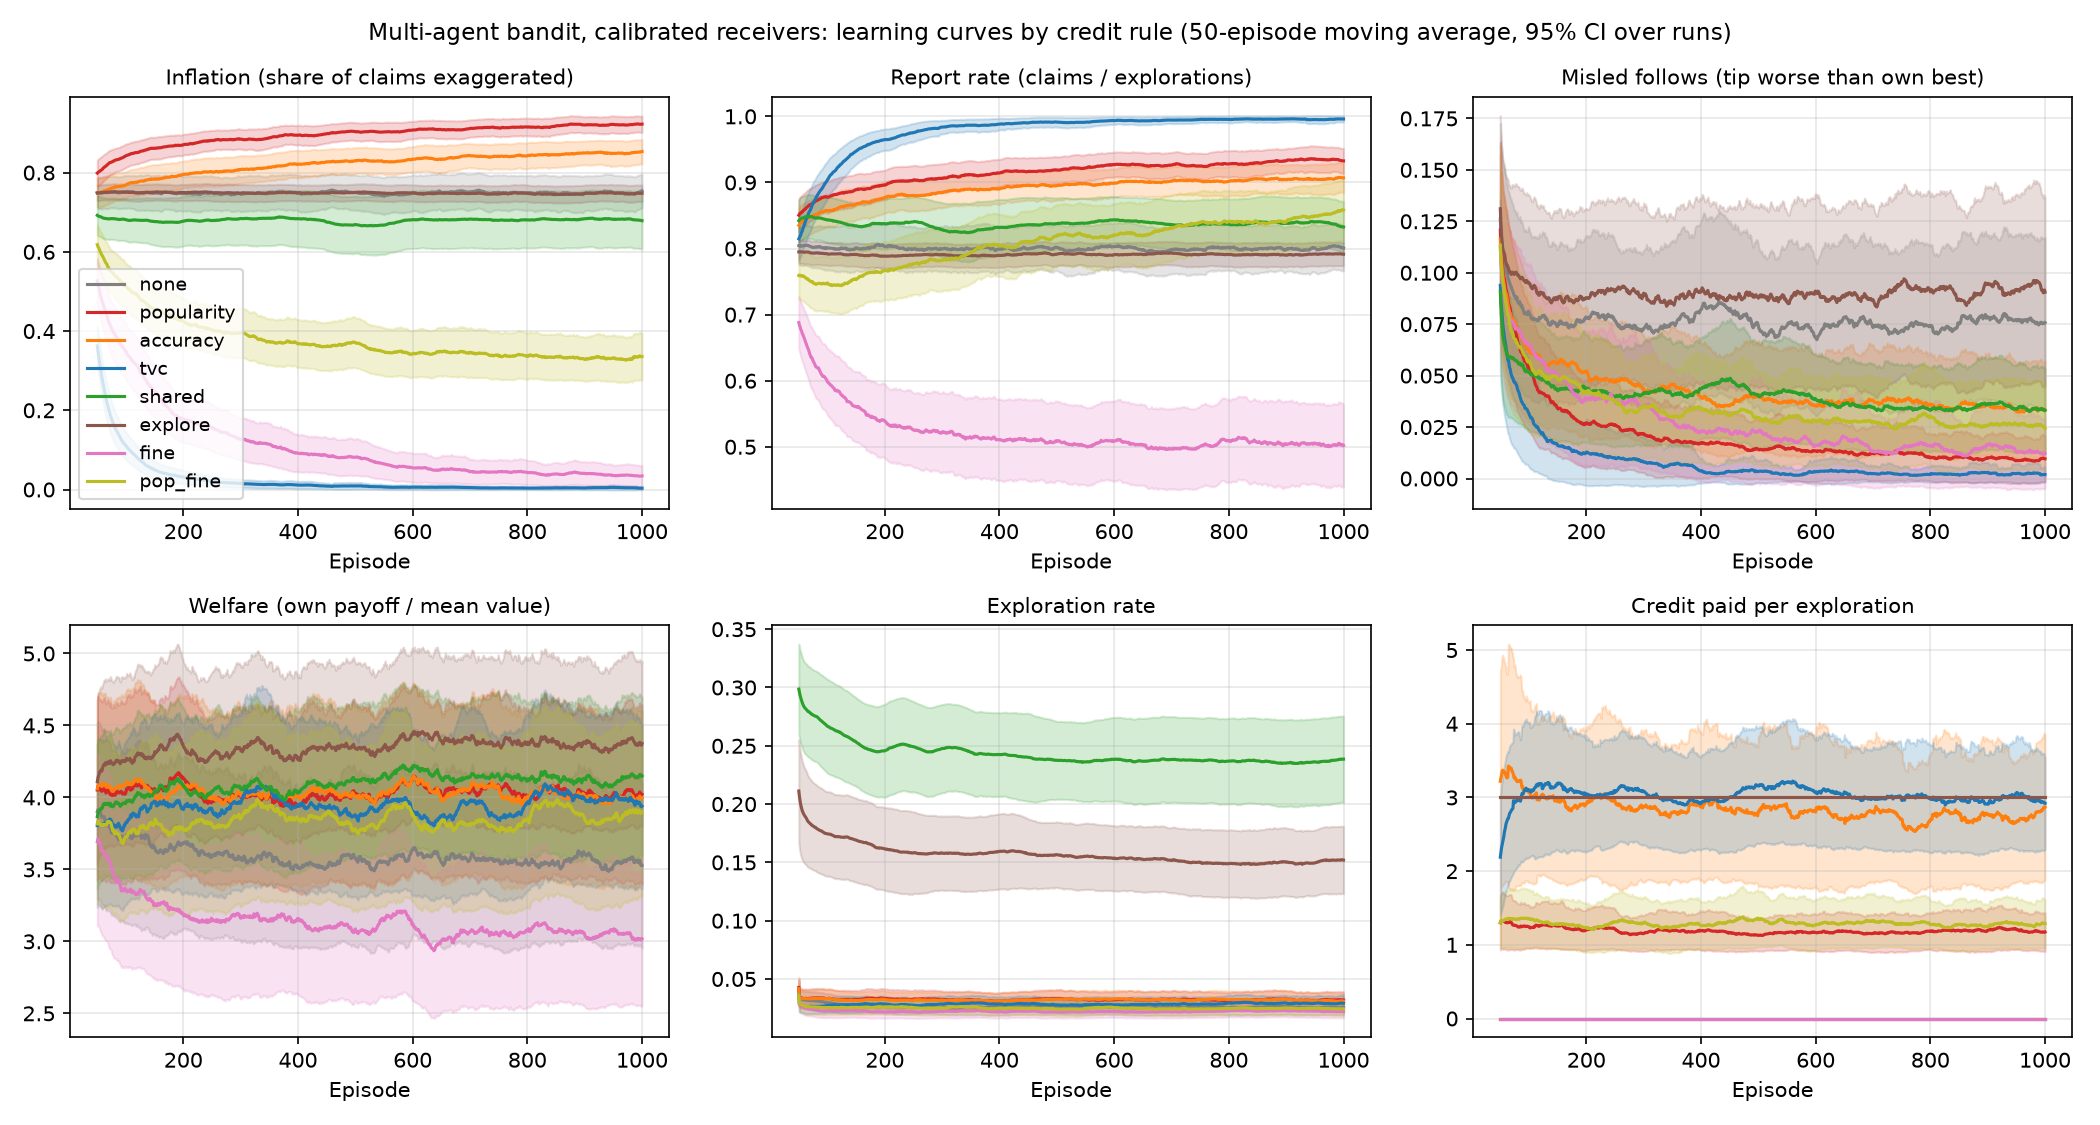
\includegraphics[width=\textwidth]{figures/bandit_calibrated.png}
%   \caption{Learning curves in the multi-agent bandit with calibrated receivers, with the same axes as \cref{fig:curves-naive}. Inflation under popularity and accuracy credit still rises slowly late in training, and under popularity credit plus a fine it still falls slowly, so the final-window means for these designs are not exact steady states.}
%   \label{fig:curves-calibrated}
% \end{figure*}

\section{Ablation Studies}
\label{app:ablation}

% \subsection{Does Lying Harm the Group?}
% To check this, we fix the claim policies instead of learning them. The first $k$ of the 12 robots post a fake jam whenever a doorway on their own route is free, the others report real jams, and no credit is given. We run 10 batches of 20 episodes for each $k$, with 95\% confidence intervals over batches. With naive receivers, group deliveries per robot per episode fall from 5.8 with no liars to 1.9 with 12 (\cref{fig:hype}), and the share of detours that were for fake jams rises from 0.31 at $k=1$ to 0.95 at $k=12$. One liar gains 3.5 deliveries over its honest peers while the others lose 0.5, so a single lie mostly moves deliveries from the others to the liar, and the group loses clearly once several robots lie. Sceptical receivers, which learn a trust for each sender from the checks they see, soften this: the group falls to 3.7 at $k=12$, and a liar's advantage at $k=1$ falls from 3.5 to 1.6. A lying robot still delivers more than an honest one at every $k<12$. Each episode starts with full trust, so this understates what trust learned over many episodes would do.

% \begin{figure*}[t]
%   \centering
%   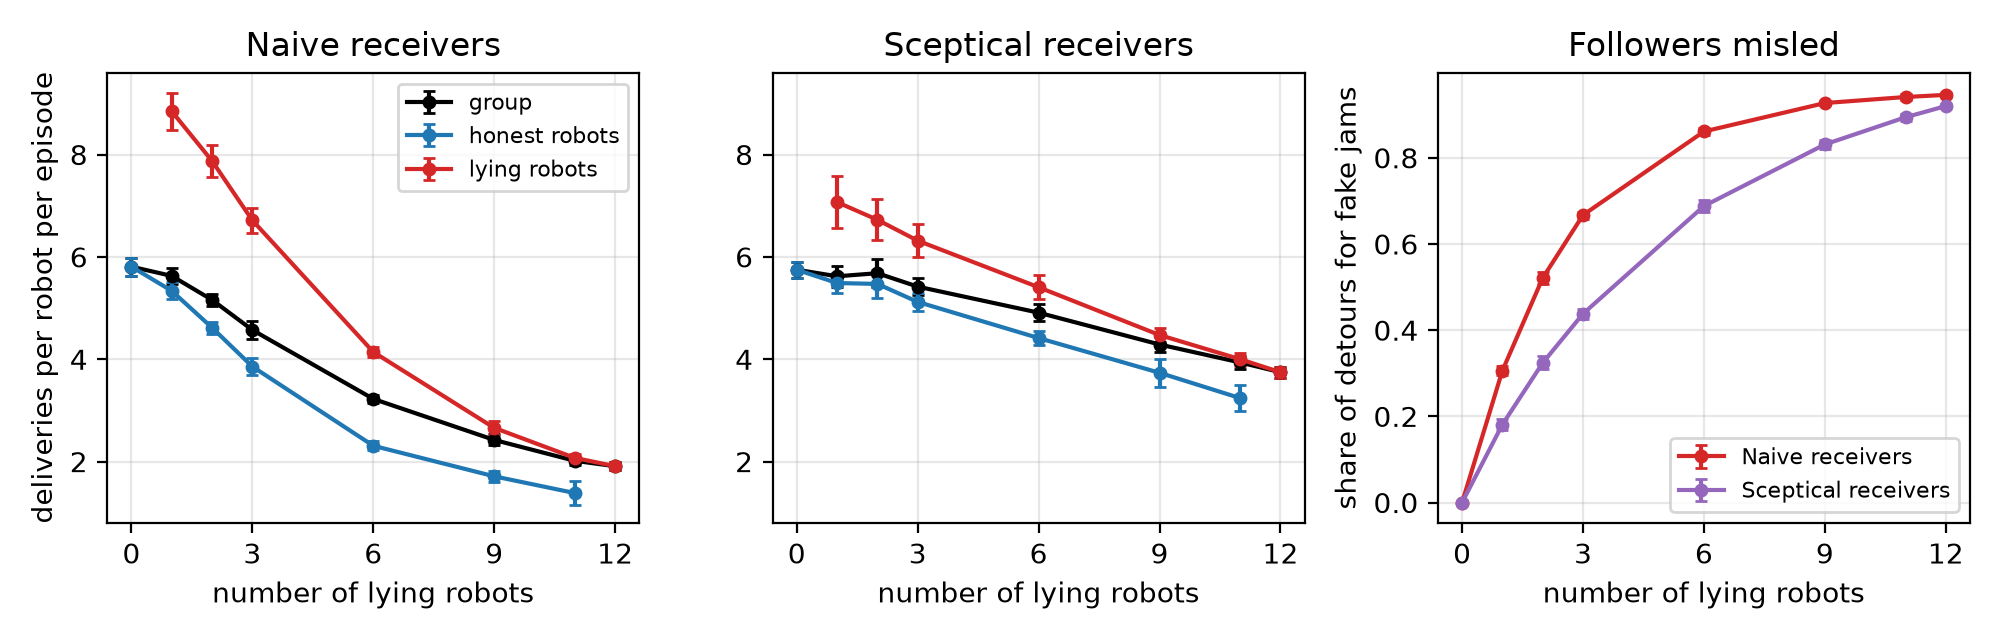
\includegraphics[width=\textwidth]{figures/fake_jams_hype_compare.png}
%   \caption{Lying harms the group in the congestion setting. The first $k$ of 12 robots post fake jams and the rest report real jams, with fixed policies and no credit (10 batches of 20 episodes, 95\% CIs). Left and middle: deliveries per robot per episode for the group, the honest robots and the lying robots, with naive and with sceptical receivers. Right: share of detours that were for fake jams.}
%   \label{fig:hype}
% \end{figure*}

% \subsection{When Do Receivers Matter?}
% To vary how much honest information changes what others do, each receiver acts on a claim only with probability $\rho$ and otherwise ignores it, with $\rho\in\{0,0.25,0.5,0.75,1\}$ and the claim policies learned as before (10 seeds). At $\rho=0$ no one acts on a claim, so a lie has no victims and an honest report helps no one, and \tvc{} adds no throughput (0.005 deliveries per robot-step with and without it, \cref{fig:listen}). Its throughput rises with $\rho$ to 0.022 at $\rho=1$, against 0.007 with no credit. Without credit the lie rate is 93--99\% whenever receivers listen, and \tvc{} holds it at 1.2\% or less at every $\rho$. The gain is not monotone at low $\rho$: at $\rho=0.25$ \tvc{} is below no credit (0.010 against 0.014). Because $\rho$ changes both whether honest information helps and whether lies have victims, this sweep does not separate the two. We therefore claim only that, in this testbed, \tvc{} raises welfare when receivers act on claims.

% \begin{figure*}[t]
%   \centering
%   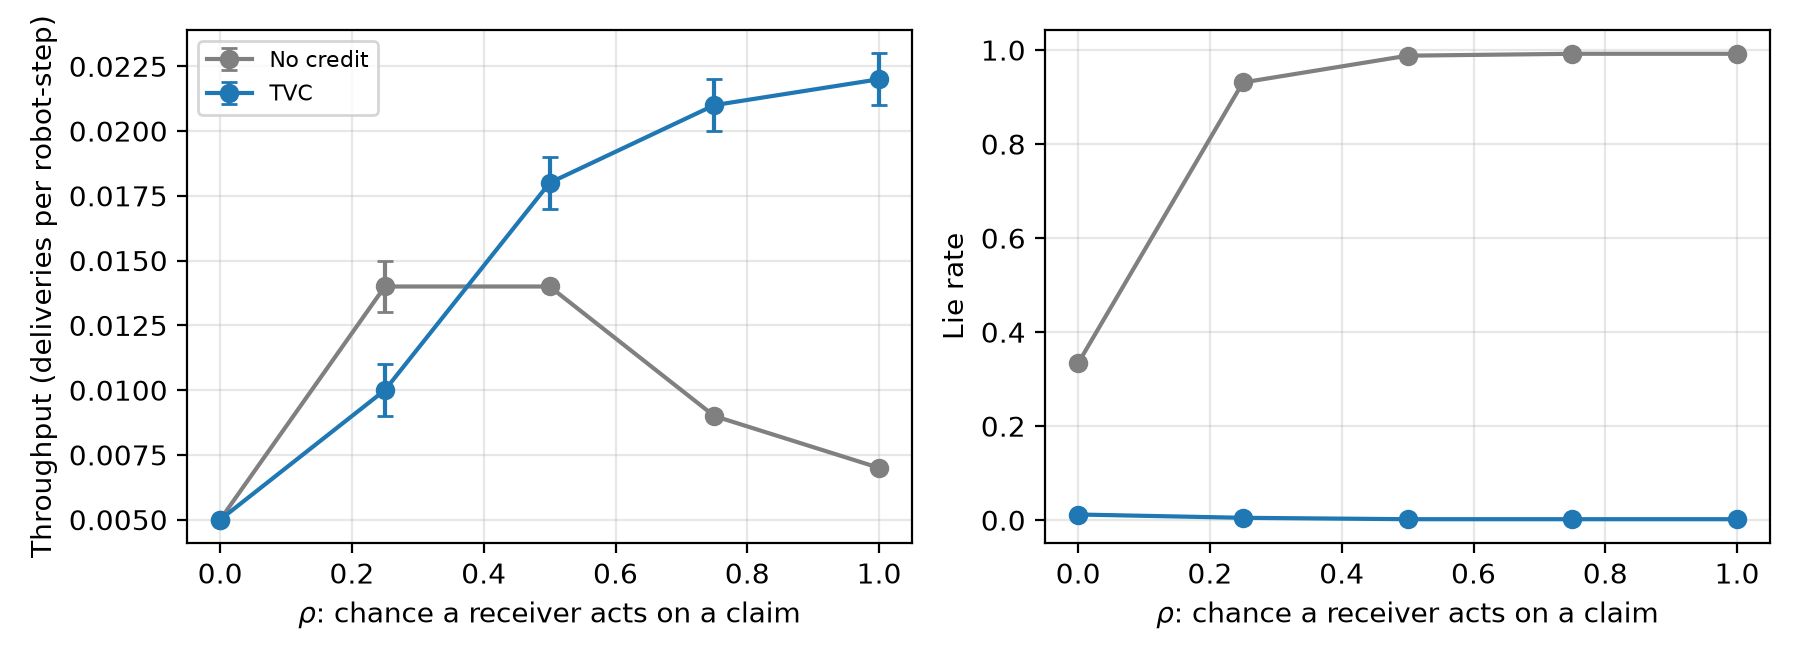
\includegraphics[width=\textwidth]{figures/fake_jams_listen.png}
%   \caption{Throughput (left) and lie rate (right) against $\rho$, the chance that a receiver acts on a claim, with no credit and with \tvc{} (10 seeds, 95\% CIs).}
%   \label{fig:listen}
% \end{figure*}

% \subsection{Which Parts of \tvc{} Are Needed?}
% We remove one part of \tvc{} at a time in the congestion setting at $\lambda=0$ (\cref{tab:ablation}; 10 seeds, 150 episodes, mean over the last 50, 95\% confidence intervals over seeds). Removing the audits ($p=0$) or the fine ($\varphi=0$) brings lying back to 99.3\% and throughput to the level of no credit. Removing the verification gate has the same effect here, because the fine is charged only on claims that fail verification, and a fake jam saves no steps, so an untruthful claim has no gain credit for the gate to block. Removing the bonus ($\eta=0$) leaves lying at 0.1\% and throughput unchanged, and lowers useful reports only slightly (96.2\% against 98.8\%), while the credit given falls from 0.040 to 0.011 per robot-step, so the bonus is not needed in this setting. Removing the cap changes nothing, because gains never reach it. This tests the parts in the congestion setting only.

% \begin{table}[t]
%   \caption{Removing one part of \tvc{} at a time in the congestion setting at $\lambda=0$ (10 seeds, mean $\pm$ 95\% CI). Lie rate and useful reports are percentages, throughput is deliveries per robot-step, and credit given is per robot-step.}
%   \label{tab:ablation}
%   \centering
%   \small
%   \setlength{\tabcolsep}{3pt}
%   \begin{tabular}{lcccc}
%     \toprule
%     Variant & Lie rate (\%) & Useful (\%) & Throughput & Credit given \\
%     \midrule
%     No credit            & $99.2 \pm 0.0$ & $44.7 \pm 1.5$ & $0.007 \pm 0.000$ & $0.000$ \\
%     Full \tvc{}          & $0.2 \pm 0.1$  & $98.8 \pm 0.7$ & $0.022 \pm 0.001$ & $0.040 \pm 0.002$ \\
%     No bonus ($\eta=0$)  & $0.1 \pm 0.0$  & $96.2 \pm 1.3$ & $0.022 \pm 0.001$ & $0.011 \pm 0.000$ \\
%     No audit ($p=0$)     & $99.3 \pm 0.0$ & $96.7 \pm 0.9$ & $0.007 \pm 0.000$ & $0.021 \pm 0.001$ \\
%     No fine ($\varphi=0$) & $99.3 \pm 0.0$ & $96.6 \pm 0.9$ & $0.007 \pm 0.000$ & $0.021 \pm 0.001$ \\
%     No gate ($\tau$ large) & $99.3 \pm 0.0$ & $96.6 \pm 0.9$ & $0.007 \pm 0.000$ & $0.021 \pm 0.001$ \\
%     No cap ($\Bbar$ large) & $0.2 \pm 0.1$  & $98.8 \pm 0.7$ & $0.022 \pm 0.001$ & $0.040 \pm 0.002$ \\
%     \bottomrule
%   \end{tabular}
% \end{table}


\end{document}
